% 原书第 177 页（PDF 第 190 页）
\BookPage{177}{190}
\BookHeading{翠华南幸扬州写真—盛清君臣眼中的扬州}{翠华南幸‧扬州写真\\[3pt]—盛清君臣眼中的扬州}{庄吉发*}
\BookSubheading{一、前言}

清朝从顺治元年（1644）满族入关确立统治政权，直到宣统三年（1911）辛亥革命清朝政权被推翻，历经二百六十八年，其中康熙皇帝在位六十一年（1662-1722），雍正皇帝在位十三年（1723-1735），乾隆皇帝在位六十年（1736-1795），这三朝皇帝在位共计一百三十四年，恰恰好占了清朝史的一半，称为盛清时期。盛清诸帝励精图治，国力兴盛，政治清明，经济繁荣，社会安定。

明成祖虽然不喜欢朱高炽，却很钟爱朱高炽的儿子朱瞻基。当廷议册立太子时，明成祖欲立汉王朱高煦。侍读学士解缙面奏明成祖说朱高炽有好儿子，明成祖有好圣孙，于是打动了明成祖的心，最后决定立朱高炽为太子，他就是明仁宗，朱瞻基就是后来的明宣宗，父子都是明朝的贤君。康熙皇帝一家三代，有些雷同。康熙皇帝虽然并不宠爱皇四子胤禛，他却十分钟爱胤禛的第四子弘历，胤禛有好儿子，康熙皇帝有好圣孙，弘历就是后来的乾隆皇帝。乾隆皇帝有好祖父玄烨，也有好父亲胤禛，而且也都是贤君。

没有雍正皇帝，清朝盛世，就无从建立。由于雍正皇帝的宵旰勤政，成功的赋役改革，终于使雍正朝的政治呈现新兴的现象，行政效率提高，严惩贪赃枉法，社会经济遂日益稳定繁荣。康熙皇帝东巡西巡，南巡北巡，多年用兵的奏销，多由雍正皇帝来善后。康熙年间的许多弊端，也由雍正皇帝来清除。雍正皇帝是促进清朝历史向前发展的关键人物。

我国历代以来，就是一个多民族的国家，满族入关后，以中华一体的政治理

\vfill
\begin{BookNotes}
\BookNote{*}{国立故宫博物院退休。}
\end{BookNotes}

% 原书第 178 页（PDF 第 191 页）
\BookPage{178}{191}
\noindent 念，破除此疆彼界的地域思想，积极消弭民族矛盾，使边疆地区与内地各省形成打成一片的完整领土，满蒙一体，满族与边疆许多少数民族已先后成为中华民族的成员。江南地区的历史背景不同，由于南明政权的统治，满汉畛域，此疆彼界的存在，亟待统治者的化解。本文尝试以康熙皇帝南巡御书留题为中心，探讨康熙皇帝赏赐御书的政治文化意义。

江南人文荟萃，自明代以来，江浙等省，不仅是经济较为富庶的地区，同时也是知识分子密集的文化中心。本文尝试以扬州等地刊刻书籍为中心，探讨盛清时期扬州等地的文化活动。

江宁织造、苏州织造、杭州织造三织造，隶内务府，掌管织造御用、内廷所用绸缎布匹及其他工艺陈设等。扬州虽然未设织造衙门，但因两淮盐政衙门设在扬州，除办理盐务外，它还兼织造、成做工艺陈设。本文尝试以扬州盐政衙门成做玉器为中心，分析扬州的玉器生产。

清朝盐课在国库收入中占有重要地位，其经营食盐购销等商人，称为盐商，包括专主收购食盐的厂商，专主行销的运商。盐商又有总商、散商之分，清朝于两淮运商中择家道殷实者为总商，其认引行销食盐的一般运商，称为散商。总商统率散商，散商行盐，须得总商具保，散商向总商纳课，由总商代缴。本文尝试以扬州盐商与科举考试为中心，说明江南乡试另编商籍的过程。

进香祈福是宗教信仰中重要的活动，清代民间进香活动，蔚为风气。江浙地区，古刹林立，各寺僧众晨钟暮鼓，顶礼金佛，虔心为皇太后诵经祈福，并祝皇帝万寿无疆。地方官员进香斋僧，为皇帝虔祝圣寿，也成为地方上重要的活动，具有正面的社会教化作用。本文尝试以扬州等地的进香活动为中心，探讨高旻寺、天宁寺、普陀山进香斋僧的宗教信仰活动。

西学的输入，中西文化的交流，天主教的传教活动，清朝政府的禁教措施，都是重要课题。本文尝试以康熙皇帝与西洋传教士的互动为中心，探讨康熙皇帝南巡期间，皇帝与江浙地区西洋传教士的对话内容，可以反映康熙中期，天主教是在一种和谐的氛围中传播福音。


% 原书第 179 页（PDF 第 192 页）
\BookPage{179}{192}
康熙皇帝关心民生，重视粮价的波动，各省督抚具折奏报雨水、收成、粮价，固然成为重要职掌，不能迟缓奏报，苏州、江宁、杭州三织造，除办理织造外，其奏报扬州等地的雨水、粮价折件，数量尤其可观。本文尝试以扬州等地粮价的波动为中心，探讨扬州等地的粮食生产与民生问题。

整饬地方吏治，改善民生，都是地方官员不容忽视的职责。扬州位处江苏适中之地，为南北往来要冲，商民聚集，政务殷繁。本文尝试以扬州府州县员缺补授为中心，说明扬州府州县官员多为精明练达之员，他们对扬州社会经济的向前发展，做出了重要贡献。

探讨御书留题，刊刻书籍，成做玉器，盐商与科举，进香祈福，康熙皇帝与西洋传教士的互动，扬州粮价的波动，整饬吏治，虽然是以偏概全，浮光掠影。但是，掌握档案，还原历史，片纸只字，也有助于对扬州的认识，对扬州学的研究，或扬州通志的纂修，确实是一种集腋成裘的工作。

二、天章炳焕·翰藻琳瑯以康熙皇帝南巡御书留题为中心

康熙皇帝在听政余暇，不分寒暑，惟以读书写字为事。他手批臣工奏折，从不假手他人，主要与他的勤习书法有关。他自己说过：

\begin{BookQuote}
朕自幼好临池，每日写千余字，从无间断。凡古名人之墨迹石刻，无不细心临摹，积今三十余年，实亦性之所好。即朕清字，亦素敏速，从无错误。凡批答督抚折子及殊笔上谕，皆朕亲书，并不起稿1。
\end{BookQuote}

康熙皇帝深悉「人君之学」不在书法，「朕非专攻书法，但暇时游情翰墨耳。2」康熙皇帝的书法，自幼即得真传。《圣祖仁皇帝庭训格言》一书记载康熙皇帝自述学习书法的经过云：

\begin{BookQuote}
朕八岁登极，即知黾勉学问。彼时教我句读者，有张、林二内侍，俱系明时多读书人。其教书惟以经书为要，至于诗文，则在所后。及至十七、八，更笃于
\end{BookQuote}

\vfill
\begin{BookNotes}
\BookNote{1.}{《十二朝东华录》，康熙朝，第2册（台北，大东书局，1968年8月），卷15，页35。康熙四十三年七月乙卯，谕旨。}
\BookNote{2.}{章侵纂《康熙政要》（台北，华文书局，据光绪刊本影印），（一)，页331。}
\end{BookNotes}

% 原书第 180 页（PDF 第 193 页）
\BookPage{180}{193}
\begin{BookQuote}
学，逐日未理事前五更即起诵读，日暮理事稍暇，复讲论琢磨，竟至过劳，痰中带血，亦未少辍。朕少年好学如此，更耽好笔墨。有翰林沈荃，素学明时董其昌字体，曾教我书法，张、林二内侍，俱及见明时善于书法之人，亦常指示，故朕之书法，有异于寻常人者以此3。
\end{BookQuote}

\par\addvspace{4pt}\noindent
\begin{minipage}[t]{0.406\linewidth}
\vspace{0pt}
\noindent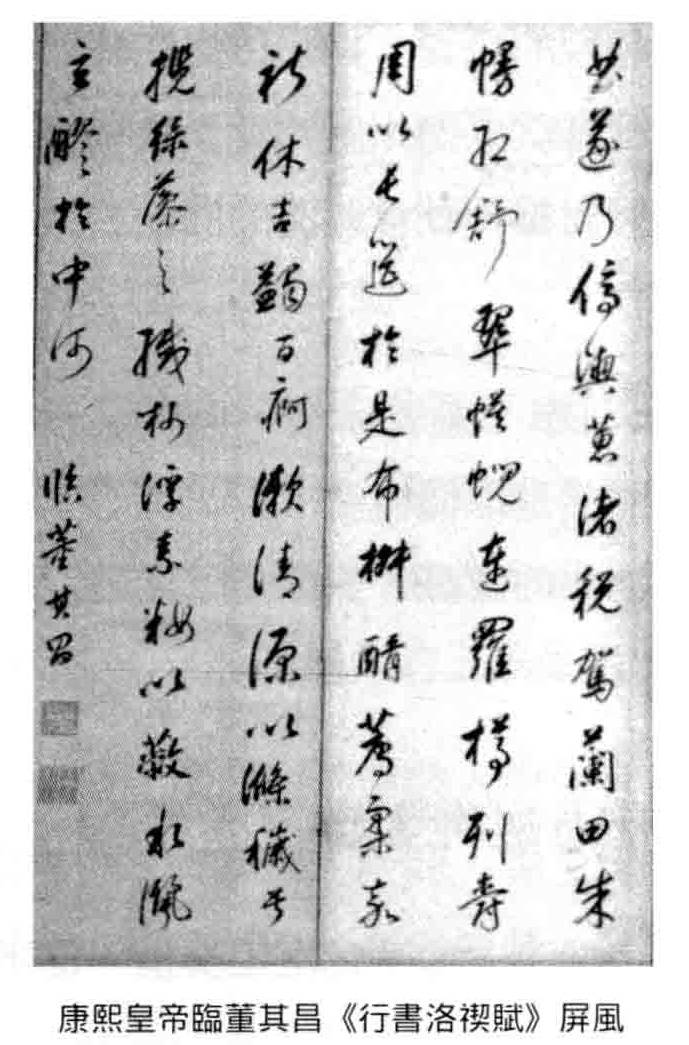
\includegraphics[width=\linewidth,height=.81\textheight,keepaspectratio]{assets/p193-01.jpg}
\end{minipage}
\hfill%
\begin{minipage}[t]{0.569\linewidth}
\vspace{0pt}\setlength{\parindent}{1.5em}
日本学者稻叶君山着《清朝全史》曾比较盛清诸帝书法，原书指出，乾隆皇帝于书法，酷爱董其昌，与康熙皇帝相似，为当时画家张得天所倾倒。乾隆皇帝的书法虽妙，似少气魄，康熙皇帝则骨力有余，丰润不足4。康熙皇帝酷爱董其昌的书法，主要是受到翰林沈荃的影响。

翰林沈荃，字贞蕤，号绎堂，江苏华亭人，其书法，为时人所倣效。闽浙总督范时崇具折奏称:「臣自幼时所写之倣，系臣父同榜进士沈荃所书，笔多带行，字如栗大。」康熙皇帝每当作书下笔时，常令沈荃侍于左右，沈

\end{minipage}
\par\addvspace{4pt}

荃即指出其缺失，并分析原因。康熙皇帝有时自书大字，令沈荃题于后。康熙十六年（1677）五月十四日辰刻，讲官喇沙里等进讲毕，沈荃进呈遵旨草书《千字文》、《百家姓》。康熙皇帝观赏过后，即将御书汉字二幅赏赐沈荃，并令喇沙里传谕说：「朕素好翰墨，以尔善于书法，故时令书写各体，备朕摹倣玩味。今将朕所书之字赐汝，非以为佳，但以摹倣尔字，故赐汝观之，果相似否。」沈荃奉到御笔后，赞叹康熙皇帝的书法，「精妙已极，实由天纵。」

\vfill
\begin{BookNotes}
\BookNote{3.}{《圣祖仁皇帝庭训格言》，见《钦定四库全书》，第717册（台北，台湾商务印书馆，1986年3月），页616-717。}
\BookNote{4.}{稻叶君山原着，但焘译订《清朝全史》（台北，台湾中华书局，1970年12月），第49章，页18。}
\BookNote{5.}{《康熙朝汉文朱批奏折汇编》，第5册（北京，档案出版社，1985年），页257。康熙五十二年十一月初五日，范时崇奏折。}
\end{BookNotes}

% 原图说　康熙皇帝临董其昌《行书洛禊赋》屏风

% 原书第 181 页（PDF 第 194 页）
\BookPage{181}{194}
沈荃曾学董其昌字体，康熙皇帝喜欢临摹其书法，沈荃又从旁指点，康熙皇帝的书法遂能「异于寻常人」。他于跋董其昌书〉中指出，「朕观昔人墨迹，华亭董其昌书昼锦堂记，字体通媚，于晋唐人中，独出新意，制以为屏，列诸座右，晨夕流览，宁不远胜镂金错彩者欤!」董其昌书法最大特色，就是高秀圆润，丰神独绝。康熙皇帝观察其结构字体后指出，董其昌书法，主要是源于晋人。康熙十六年（1677）十一月二十二日，康熙皇帝亲跋〈王右军书曹娥碑真迹〉云:「曹娥碑相传为晋王右军将军王羲之得意书。今覩真迹，笔势清圆秀劲，众美兼备，古来楷法之精，未有与之匹者。至今千余年，神彩生动，透出绢素之外。朕万几余暇，披玩摹倣，觉晋人风味，宛在几案间，因书数言识之。」王羲之曹娥碑真迹，笔势清圆秀劲，确实是希代珍宝，千余年来，依然神彩生动，康熙二十一年（1682）二月初八日，康熙皇帝〈跋董其昌书〉指出，以屏风装潢告成，尙余缣素，詹事沈荃也是华亭人，与董其昌同乡，又素学董其昌笔法，于是命沈荃续书题跋。沈荃之子沈宗敬，亦善书法，沈荃卒后，沈宗敬以编修入直南书房，康熙皇帝命作大小行楷，犹意其父沈荃，曾谕大学士李光地称:「朕初学书，宗敬父荃，指陈得失，至今作字，未尝不思其勤也8。」由此可知康熙皇帝喜欢董其昌的书法，主要是受到沈荃的影响。

康熙皇帝南巡期间，在行宫读书写字，每至深夜，乐此不疲，所到之处，御书留题，颇具历史文化意义。康熙二十三年（1684），康熙皇帝首次南巡。《南巡笔记》记载，是年「秋九月，陈请两宫，暂违定省。二十八日，出京师，经河间，过德州，阅济南城，观趵突泉，题曰激湍”。」《起居注册》记载较详，是年九月二十八日，康熙皇帝由午门出正阳门，驻跸永清。同年十月初八日，驾至济南府趵突泉亭，临泉览视，称赏不已。山东巡抚徐旭龄奏请御笔留题。康熙皇帝以趵突泉为名胜之地，即援笔大书「激湍」二字。侍讲学士高士奇等扈从诸臣、山东巡

\vfill
\begin{BookNotes}
\BookNote{6.}{《清圣祖御制文初集》，故宫珍本丛刊，第543册（海口，海南出版社，2000年6月），卷28，页10。}
\BookNote{7.}{《清代起居注册》，康熙朝，第5册（北京，中华书局，2009年9月），页B002414。康熙十六年十一月二十二日，跋曹娥碑真迹词。}
\BookNote{8.}{《清史稿校注》，第11册（台北，国史馆，1989年2月），沈荃列传，页8575。}
\BookNote{9.}{《清圣祖御制文初集》，卷20，页5。}
\end{BookNotes}

% 原书第 182 页（PDF 第 195 页）
\BookPage{182}{195}
\noindent 抚徐旭龄瞻仰御书后赞叹御书神妙，真有「龙跳凤舞之势」，山泉生色。康熙皇帝命扈从诸臣各书二字留之泉亭，以传来许。一鼓后，侍卫二格捧出御书「清漪」二字赐诸臣观览。因山东巡抚徐旭龄以衙署内有珍珠泉，奏请御书留题，康熙皇帝即以「清漪」二字赐之。大学士明珠等瞻仰宸翰后指出，御书笔墨飞舞，备极其妙，「清漪」二字，意义尤美1°。同年十月十一日早，康熙皇帝率从官登泰山，于天仙殿行礼，御书「坤元叶德」四大字，悬额殿中。回行宫后，将御书「普照乾坤」四大字、「云峰」二大字，宣示从臣。扈从诸臣瞻仰后指出，御书笔力雄健，结撰精整。康熙皇帝谕令将「普照乾坤」四大字于孔子小天下处建亭悬额，「云峰」二字，则令于泰山极顶处磨崖勒石。

康熙二十三年（1684）十月二十二日，康熙皇帝驾幸扬州后，登览蜀冈楼灵寺平山堂等名胜，御书「怡情」二字，留题于平山堂。康熙皇帝驾幸天宁寺时，御书「萧闲」二字。十月二十四日，康熙皇帝乘沙船渡扬子江。次早，登金山游龙禅寺，御题「江天一揽」四字11。十月二十八日，驾幸苏州观惠泉山。是日，康熙皇帝以苏州乡官汪琬原系翰林，为人厚重，学问优通，且居乡安静，不预外事，因此，特赐御笔手卷一轴。同年十一月初四日，康熙皇帝亲书手卷一轴赐江宁府知府于成龙。是日，令大学士明珠传谕于成龙曰：

\begin{BookQuote}
朕于京师即闻尔知府于成龙居官廉洁，今临幸此地，咨访与前所闻无异，是用赐尔朕亲书手卷一轴。朕所书字，非尔等职官应得者，特因嘉尔清操，以示旌
\end{BookQuote}

扬12。

康熙皇帝虽然重视书法，勤于写字，但是他不轻易亲书赏赐品级较低职官。

康熙二十八年（1689）正月初八日，康熙皇帝第二次南巡。是日黎明自午门出正阳门。正月十三日，驻跸山东德州西关。康熙皇帝曾撰孔子、孟子及周公庙碑文各一篇，手书勒石。衍圣公孔毓圻等奏请御书墨本以为世宝，因此，命将孔子、孟子、周公庙碑文装潢成册，分赐衍圣公孔毓圻、博士孟贞仁等。正月十六日辰刻，

\vfill
\begin{BookNotes}
\BookNote{10.}{《清代起居注册》，康熙朝，第17册，页B008359。康熙二十三年十月初八日，记事。}
\BookNote{11.}{康熙二十三年十月二十四日，康熙皇帝乘沙船渡过扬子江临幸金山游龙禅寺题字，《起居注册》作「江天一揽」四字，《清圣祖御制文初集·南巡笔记》作「江天一览」。}
\BookNote{12.}{《清代起居注册》，康熙朝，第17册，页B008422。康熙二十三年十一月初四日，谕旨。}
\end{BookNotes}

% 原书第 183 页（PDF 第 196 页）
\BookPage{183}{196}
\noindent 驾进济南府，因访民俗之便，观赏趵突、珍珠二泉。扈从诸臣及山东巡抚钱珏等公请御笔留题为名泉光宠，康熙皇帝御亭书写「作霖」二大字。

康熙皇帝因禹王庙礼器简少，屋宇倾颓，特撰上谕，亲至禹王庙致祭。康熙二十八年（1689）二月十六日，驻跸杭州府行宫，亲书「地平天成」四字，悬挂于禹王庙宇下，并着地方官修理庙宇。同年二月二十九日，康熙皇帝以两江总督傅腊塔、将军博济、江南提督将军杨捷同效勤劳，故手书御制诗赐之。傅腊塔等均表示铭诸肺腑，戴恩图报。

康熙三十八年（1699），康熙皇帝第三次南巡。是年二月初三日凌晨，由东华门出崇文门至大通桥登舟，过通州。二月初四日，驻跸新河长乐营地方。是日，赐直隶巡道赵弘燮御书「清惠不群」四大字，并传谕曰:「尔父赵良栋矢志报国，克弹勤劳，历事戎行，茂着勋绩，朕迄今犹追念之，以尔兄弟系功臣之子，未必玷辱先人，故皆擢用，授以文武要职。今复以此四字赐汝，此后益当砥砺廉洁，广宣惠爱，以副朕视民如子之至意。」二月初十日，康熙皇帝过沧州，驻跸砖河地方。是日，赐管理绎夫礼部员外郎舒古鼐、慎刑司员外郎阿尔赛御书各一幅。二月十一日，驻跸东光县夏口地方。是日，赐管理绎夫郎中穆楚库、员外郎常代御书各一幅

康熙三十八年（1699）二月十二日，康熙皇帝驻跸桑园地方，赐天津总兵潘育龙御书《杜若赋》一幅、《渊鉴斋法帖》一部；直隶巡抚李光地《耕织图》一册、《渊鉴斋法帖》一部、守道高必弘、巡道赵弘燮、天津道范时崇、通永道祝兆熊等俱赐《耕织图》一册。二月十三日，驻跸洛坡屯地方，赐管绎夫员外郎满蒲、阿迷达御书各一幅。二月十八日，驻跸两响闸地方。原任刑部侍郎任克溥来朝，赐御书「冰壶朗印」四大字，临米芾《天马赋》一卷，又赐尚芝龙、张鼎臣、张鼎鼐、张常住御书各一幅。二月二十四日，驻跸赤山，赐山东巡抚王国昌、布政使刘瞪、按察使李基和《渊鉴斋法帖》各一部。

康熙三十八年（1699）三月初四日，驻跸淮安府城。是晚登舟，赐总漕桑格激引清风」四大字，墨刻《金刚经》、《龙虎台赋》手卷、《秋清赋》、《耕织图》各一册。三月初八日，驻跸扬州府城内。赐原任工部侍郎李柟御书「多识畜


% 原书第 184 页（PDF 第 197 页）
\BookPage{184}{197}
\noindent 德」四大字、对联一副、唐诗一幅；赐原任布政使汪楫「游咏清风」四大字，并字一幅；原任给事中李宗孔亦赐「游咏清风」四大字，并字一幅；赐扬州府天宁寺僧广元御书「禅心澄水月」五大字、「佛门堂」三大字、「皓月禅心」四大字、「寄怀闲竹」四大字；赐兴教寺僧广彻「西来法」三大字；赐北峙僧广证「法律禅」三大字。三月初九日，驻跸江天寺，赐粮道刘德芳御书「龙飞」二大字、「扬仁风三大字、并字一幅、手卷一轴；凤庐道佟毓秀、扬州府知府傅泽洪赐御书字各一幅；赐扬州盐商张文秀御书「松风」二大字、手卷一轴；赐天宁寺僧广元御书「鹰堂」二大字；赐北来寺僧「上崇」二大字、「慈云」二大字。三月十一日，驻跸兴丰，赐江天寺僧超乐御书《心经》，并字四幅；赐僧明真御书「云峰」二大字，「松风石」三大字、并字一幅；赐避风馆僧源恒御书「甘露门」三大字、《金刚经》一部；赐僧明融御书「超峰」二大字、经一部；赐僧妙觉御书「禅栖」二大字、经一部；赐僧僧澜御书「善觉」二大字、经一部；赐僧慧光等九人经各一部。三月十三日，驻跸无锡县，赐管夫广储司郎中皂保、掌仪司员外郎陶朱、户部员外郎敦多御书各一幅。

康熙三十八年（1699）三月十五日，驻跸苏州府城内。是日，康熙皇帝御笔临董其昌书「家鸡野骛春蚓秋蛇」八大字，命中使赍示掌院学士韩菼。韩菼奏曰:「皇上御笔书法，不啻龙飞凤舞，晋唐名迹所不及，何况其昌。」因此，奏请赏赐御书八字，奉为永宝。中使入奏，随后中使捧出御书「东南云峰」四大字，并赐御书「家鸡野骛春蚓秋蛇」八大字。韩菼瞻仰「东南云峰」四大字后指出，御书笔法超绝，于是奏请勒石虎丘，以彰荣遇。三月十六日，驻跸苏州府。是日，赐江苏巡抚宋荦御书「仁惠诚民」四大字、「怀抱清朗」四大字、临米字一幅、《天马赋》一卷、诗扇一柄、《渊鉴斋法帖》一部、《耕织图》一部；赐提督张云翼御书「思无邪」三大字、字一幅、手卷一幅、诗扇一柄、《渊鉴斋法帖》一部、《耕织图》一部。三月十八日，驻跸苏州府，赐两江总督张鹏翮御书一幅。三月十九日，驻跸苏州府。赐苏州织造李煦御书「修竹清风」四大字、字二幅；赐原任尚书翁叔元墨刻《金刚经》、《孝经》、《草诀百韵歌》、《耕织图》、御书诗扇字三幅；赐原任尚书王日藻墨刻《金刚经》、《孝经》、《草诀百韵歌》、《耕织图》，并御书「连云」二大字、字三幅。赐原任御使徐树谷墨刻《金刚经》、《孝经》、《草诀


% 原书第 185 页（PDF 第 198 页）
\BookPage{185}{198}
\noindent 百韵歌》、《耕织图》、御书「天光云影」四大字、字二幅；赐原任巡抚顾汧墨刻《金刚经》、《孝经》、《草诀百韵歌》、《耕织图》、御书诗扇字；赐原任国子监典簿徐升《耕织图》、御书「云光台」三大字、字一幅；赐原任给事中慕琛墨刻《金刚经》、《孝经》、《草诀百韵歌》、《耕织图》、御书字二幅；赐原任庶吉士沈宗敬《孝经》、墨刻《千字文》、御书「清风兰雪」四大字、字一幅。因扈从汉翰林官中多苏松人，康熙皇帝令奏事存住传谕苏松翰林官可就近到家与父母妻子相见，不必随驾至浙江。三月二十日，驻跸皂林，赐苏州云泉寺僧持藻御书「般若台」三大字。

康熙三十八年（1699）三月二十六日，驻跸杭州府。是日，赐浙闽总督郭世隆御书「岳牧之任」四大字，手卷一幅、《渊鉴斋法帖》、《耕织图》；赐浙江巡抚张敏御书「宣布德泽」四大字，手卷一幅、《渊鉴斋法帖》、《耕织图》；赐提督赵弘灿御书「乐善不倦」四大字、《耕织图》、《渊鉴斋法帖》；三月二十七日，驻跸杭州府。是日，亲近侍卫伍什、学士布泰捧出御书「名垂青史」四大字赐浙江湖州府知府陈一夔，并传谕曰:「尔父陈丹赤向为国尽忠殉难，朕至今悯之，此赐特表尔父之忠耳。」同日，赐福建将军金世荣御书「器志方雅」四大字；赐提督王万祥御书「智义合宜」四大字；赐总兵官御书「惠迪吉」三大字；赐蓝理御书「所向无前」四大字；赐内阁学士胡会恩御书「秘阁清班」四大字；赐庶子陈元龙御书「凤池良彦」四大字、字一幅；赐南海普陀山僧明志御书「潮音洞」三大字、「梵音洞」三大字、「普济群灵」四大字、「浩月禅心」四大字、字一幅；赐僧性统御书「天花法雨」四大字、「修持净业」四大字、字一幅；赐天竺寺僧挺萃御书「法云慈悲」四大字；赐僧辂慧御书「飞来峰」三大字、「云栖」二大字，命镌悬二处。三月二十八日，驻跸杭州府城。是日，赐内阁学士顾祖荣御书「邃清之秩」四大字；赐副都御史吴涵御书「风霜之任」四大字；赐布政使赵良璧「承流宣化」四大字；赐按察使于准廉御书「廉察之寄」四大字；赐净持寺僧方孝御书「西峰」二大字及对联一副。三月二十九日，赐杭州织造官敖福合御书「鸾鹤情」三大字、「兰亭」二大字、对联一幅、字一幅；赐驿盐道卞三畏御书「廉镇」二大字；赐原任詹事府詹事高士奇御书「忠孝节义」四大字、对联一副、字一幅；赐原任少詹事邵远平御书「蓬观」二大字；赐原任谕德沈涵御书「华省」二大字；赐原任中允蔡


% 原书第 186 页（PDF 第 199 页）
\BookPage{186}{199}
\noindent 升元御书「清华」二大字；赐原任御史龚翔麟御书「兰台」二大字；赐原任总督甘文焜之子同知甘国奎御书「劲节」二大字；赐玉泉禅寺僧等裕《金刚经》。

\par\addvspace{4pt}\noindent
\begin{minipage}[t]{0.221\linewidth}
\vspace{0pt}
\noindent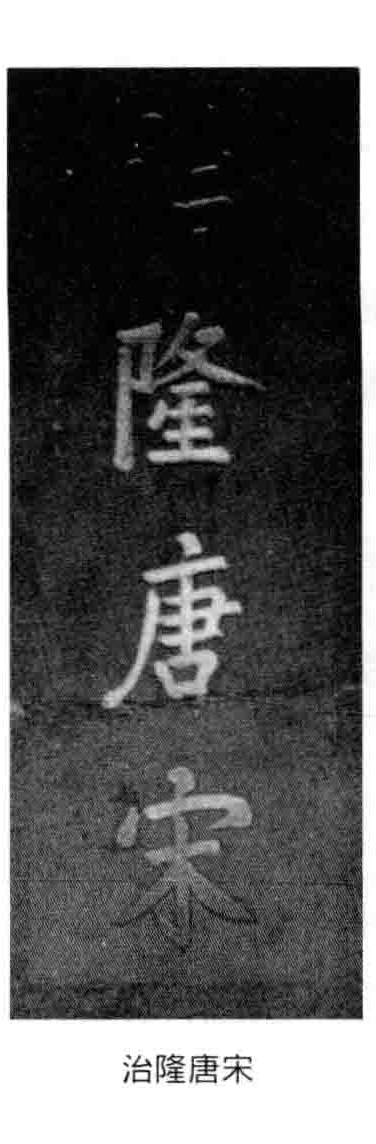
\includegraphics[width=\linewidth,height=.81\textheight,keepaspectratio]{assets/p199-01.jpg}
\end{minipage}
\hfill%
\begin{minipage}[t]{0.754\linewidth}
\vspace{0pt}\setlength{\parindent}{1.5em}
康熙三十八年（1699）四月初二日，驻跸苏州府。康熙皇帝因念原任大学士宋德宜，御书「笃念前劳」四大字赐其子给事中宋骏业、赞善宋大业，又赐宋骏业御书「蹇谔老成」四大字，赐宋大业御书「文学侍从」四大字。同日，赐翰林院侍讲学士王九龄御书「视草」二大字；侍读学士张廷瓒御书「玉堂」二大字；国子监祭酒孙岳颁御书「尊经服教」四大字；原任侍郎彭孙遹御书「松桂堂」三大字；百岁老人顾履吉御书「凌雪乔松」四大字；九十二岁老人褚篆御书「海鹤风姿」四大字。四月初五日，驻跸苏州。是日，赐原任尚书翁叔元御书「揽秀堂」三大字；赐原任詹事高士奇御书「再过鹅峰」四大字；赐给事中宋骏业「御制悯农诗」一章及御书，宋骏业奏准勒石学宫；赐原任御史盛符升御书「年登大耋」四大字；赐原任赞善黄与坚御书「如松堂」三大字；赐原任检讨尤恫御书「鹤栖堂」三大字；赐原

\end{minipage}
\par\addvspace{4pt}

\noindent 任廵抚顾汧御书「阅清晖」三大字；赐两浙运使道李涛御书「惠爱」二大字；赐织造府官李煦御题诗一首，对联一副；赐江晖之子江弘文墨刻《千字文》、《诗经》各一本；赐华山和尚敏膺御书「高云」二大字。「翠𪨷寺」三大字、字一幅；赐祥符寺僧纪荫御书「神骏寺」三大字。四月初六日，康熙皇帝自苏州府起行，驻跸望亭。是日，赐杭州司库戚色御书一幅；赐华山和尙敏膺御书「香域」二大字。四月初七日，驻跸定堰地方。是日，赐原任左春坊秦松龄御书「松风水月」四大字、「山色溪光」四大字；赐放生池和尚御书「慈云寺」三大字；赐小金山和尚御书「兰若」二大字。四月初八日，驻跸丹阳地方。是日，赐和尚纪荫御书「清净寺」三大字、字二幅、对聨一副。四月十四日，驻跸江宁府赐浙江布政使赵良璧、按察使于准，驿传道卞三畏、盐运使李涛《渊鉴斋法帖》、《耕织图》。

康熙三十八年（1699）四月十五日，康熙皇帝命大学士伊桑阿等赍送御书「治隆唐宋」四大字、黄绫一幅至洪武陵，陈设香案行礼，将御书交与织造府官曹寅收


% 原图说　治隆唐宋

% 原书第 187 页（PDF 第 200 页）
\BookPage{187}{200}
\noindent 贮，俟修理完毕悬挂。是日，赐安徽廵抚李御书「敷政于外」四大字；赐安徽布政使张四教御书「忠信之长」四大字；赐江苏布政使刘殿衡御书「藩维之寄」四大字；赐江苏按察使赵世显御书「清明仁恕」四大字；赐苏松粮道刘殿邦御书「一州之表」四大字；赐驿盐道王然御书「清简为最」四大字；赐安徽粮道鲍复昌御书「治民如家」四大字；赐凤庐道佟毓秀御书「惠爱在人」四大字；赐常道施朝辅御书「百里宣风」四大字。以织造府官曹寅之母年老，特赐御书「萱瑞堂」三大字，赐曹寅御书「云窓清霭」四大字、字一幅、对联一副、《渊鉴斋法帖》一部；赐苏州府织造官李煦《渊鉴斋法帖》；赐报恩寺僧法镇《金刚经》一部。

康熙三十八年（1699）四月二十日，驻跸金山。是日，赐大学士张玉书御书「恭俭为德澄怀日新」八大字、「浮翠楼」三大字、字一幅、对聨二副、《渊鉴斋法帖》、《耕织图》；赐总河于成龙御书「澄清方岳」四大字、字二副、对联一副；赐镇江僧广如御书「八公洞」三大字、《金刚经》一卷；赐超着御书「鹤林寺」三大字、《金刚经》一卷；赐超学御书「竹林寺」三大字、《金刚经》一卷；赐江天寺僧深起御书「水天清映」四大字；赐印铨御书「清规」二大字；赐僧湛悟《金刚经》一卷。四月二十二日，驻跸扬州府。赐原任给事中李宗孔御书「香山洛社」四大字；赐原任侍郎李柟御制诗一幅；赐两淮盐院卓琳御书「紫垣」二大字；赐原任主事郭士璟御书「泉石怡情」四大字；赐御史程文彝御书「肃纪守法」四大字；赐原任道程兆麟御书「歌咏昔贤」四大字；赐芜湖关监督翰林院侍讲学士郎启御书「竹风兰露」四大字；赐原任尚书徐干学之子原任御史徐树谷御书「爱清景」三大字；赐原任詹事沈荃之子原任庶吉士沈宗敬御书「落纸云烟」四大字；赐盐商项起鹤母「寿萱」二大字；赐盐商汪森裕御书「礼年高」三大字；赐举人吴廷祯字一幅；赐天宁寺僧广元御书诗一章；赐清凉寺僧纪荫御书一幅；赐焦山僧御书「法云惠日」四大字；赐天心寺僧元启御书「香阜寺」三大字、《金刚经》一卷；赐万佛庵僧普怡「云门雪窦」四大字、《金刚经》一卷。

康熙三十八年（1699）四月二十四日，驻跸汛水地方。是日，赐相士罗光荣御书「通幽索隐」四大字；赐江天寺僧「龙光寺」三大字；赐南京兴善寺僧明融《金刚经》一卷。四月二十五日，驻跸淮安城外。是日，赐内阁学士布泰御书「木天」


% 原书第 188 页（PDF 第 201 页）
\BookPage{188}{201}
\noindent 二大字；赐苏州府云泉寺僧特藻御书「慧业寺」三大字、「精舍」二大字、《金刚经》二卷。四月二十八日，驻跸治河嘴地方。是日，赐于成龙御书「乐休祉」三大字、对联一副；赐徐廷玺御书「慈惠之师」四大字；赐云台寺僧隆祯御书「遥镇洪流」四大字。

康熙三十八年（1699）五月初一日，驻跸韩庄闸是日，赐原任詹事高士奇御墨五匣。五月初三日，驻跸仲家闸。是日，赐五经博士仲秉贞御书「圣门之哲」四大字，命悬于子路庙。五月初六日，驻跸李海务。是日，赐原任詹事高士奇御书条幅、对聨、《渊鉴斋法帖》、《百家姓》、《千字文》、《草诀百韵歌》、《金刚经》墨刻、《耕织图》；赐大名府九十七岁老人聂志笙御书「春秋高」三大字；赐直郡王御书「绮窓」二大字；赐诚郡王「拥书千卷」四大字、「芸窓」二大字、「云舫」二大字；赐七贝勒御书「进学斋」三大字；赐衍圣公孔毓圻御书「诗书礼乐」四大字；赐五经博士孔毓埏御书「远秀」二大字；赐山东廵抚王国昌御书「珪璋特达」四大字；赐山东布政使刘皑御书「维德之隅」四大字；赐山东按察使李基和御书「独持风裁」四大字；赐登莱道郎廷极御书「振鹭初飞」四大字；赐原任侍郎任克溥御制诗一篇、御书「传世宝」三大字13。五月初十日，驻跸白草洼。是日，赐裕亲王御制诗一章。五月十三日，驻跸张家庄。是日，赐天津总兵官潘育龙御书「尽锐争先」四大字。五月十四日，驻跸河西务。是日，赐内阁学士噶礼御书「清班」二大字；赐管夫郎中马尔汉、常有、员外郎恩爱御书各一幅。五月十六日，驻跸通州城外，赐兵部尚书席尔达御书「居贞素」三大字及字一幅。五月十七日，是日早，康熙皇帝由崇文门进东华门回宫。

康熙四十一年（1702）九月二十五日辰时，康熙皇帝因廵视南河，由午门出正阳门南廵。十月初四日，驻跸德州城。初五日，驻跸行宫，皇太子违和。是日巳时，命侍读学士陈元龙、侍讲学士揆叙、侍读宋大业、谕德查升、编修汪士、陈壮履、庶吉士励廷仪入行宫赐食。饭后，召陈元龙等至御前，令各书绫一幅。起居注册详录君臣讨论书法的对话，节录一段内容如下：

\begin{BookQuote}
上阅毕云：励廷仪书法甚熟，因在朕前，过于矜持，是以不及平昔。上又曰：
\end{BookQuote}

\vfill
\begin{BookNotes}
\BookNote{13.}{《清代起居注册》，康熙朝，第13册，T07143。康熙三十八年五月初六日，据任克溥奏。}
\end{BookNotes}

% 原书第 189 页（PDF 第 202 页）
\BookPage{189}{202}
\begin{BookQuote}
学书须临古人法帖，其用笔时，轻重疏密，或疾或迟，斟酌俱有体。宫中古法帖甚多，朕皆临阅。有李北海书华山寺碑文，字极大，难于临摹。朕身临其上必临摹而后已。今翰林内书法优者，皆有一种翰林习气，惟孙岳颁书法最佳。查升奏曰：孙岳颁草书、楷书俱佳。上曰：孙岳颁楷书亦未免有翰林气，其草书实是过人。陈元龙等奏曰：臣等蒙圣恩训示，虽曾究心书法，但古人法帖，其运笔结构，皆未能辨晰。皇上御书超绝千古，纵锺繇、王羲之复生，皆不能及。臣等蒙皇上赏赉御书，虽朝夕瞻仰，心摹手习，一笔亦不能学，总由圣躬干健，腕力万钧，洵圣寿无疆之征也。臣等鲁钝，愿学未能，况御札精微奥妙，又非臣等愚昧所能仰窥。今驻跸闲暇，蒙恩召进，臣敢冒昧丐求皇上亲挥御笔，许臣等侍侧，恭瞻皇上用笔之妙，书法之神，庶几窥窃万一，以仰副皇上教育鸿恩，臣等曷胜激切之至。皇上遂亲书『云飞北阙轻阴散雨歇南山积翠来』十四大字，真如龙飞凤舞，岳峙渊停，诸臣拱立，钦仰懽忭，赞飏难罄焉。上又曰：米芾石刻，可不必学，所有法帖，朕曾临徧，大抵名人墨迹，屡经匠工镂刊，其原本精神，渐皆失真。沈荃昔云：伊曾亲受董其昌指训。朕幼年学书，有一笔不似处，沈荃必直言之。朕素性好此，久历岁年，毫无间断14。
\end{BookQuote}

侍读学士陈元龙等对康熙皇帝书法的肯定，虽多溢美之辞，但君臣重视书法的重要性，确实是不言可喻。引文中指出康熙皇帝临遍清宫珍藏古人法帖，以及如何临摹古人法帖，都是经验之谈。米芾书法，颇得王献之笔意，超妙入神。但因米芾墨迹屡经匠工镂刊，以致失真，而无原本精神，米芾石刻不必学，康熙皇帝的分析是可信的。因皇太子染病，南廵中辍。十月二十一日，皇太子病体大愈，康熙皇帝于是日回銮。

康熙皇帝不仅以御书赏赐臣工，亦常赏赐宝砚。康熙四十二年（1703）正月初三日早，康熙皇帝召翰林院掌院学士揆叙等六十人至南书房，赏赐砥石山石砚，人各一方，就是「作养词臣」的一种表现。同年正月十六日，康熙皇帝以廵阅南河，省风问俗，察访吏治，于是日巳时由畅春园启行，驻跸良乡县所属窦店，御书《督抚箴》一篇赐直隶巡抚李光地。正月十八日，驻跸河间府属临河地界，赐分司

\vfill
\begin{BookNotes}
\BookNote{14.}{《清代起居注册》，康熙朝，第17册，T09624。康熙四十一年十月初五日，谕旨。}
\end{BookNotes}

% 原书第 190 页（PDF 第 203 页）
\BookPage{190}{203}
\noindent 齐苏勒御书诗一幅。正月二十四日，康熙皇帝至济南府，幸廵抚署中观珍珠泉，御书《三渡齐河即事诗》一章，令悬于大门，晓示臣民。又书《督抚箴》一篇及御制诗，赐山东廵抚王国昌。复出观趵突泉，驻跸长清县属黄山店，御书「源清流洁」四大字，令悬于趵突泉。又书「润物」二大字，令悬于珍珠泉。又书「学宗洙泗四大字，令悬于学道所修书院。正月二十六日，驻跸泰安州城内。二月初七日，御舟过高邮州，泊舟邵伯。是日，过邵伯更楼，至扬州登岸，经过城内，阖城士庶，扶老携幼，设香案，争覩「天颜」。同日，出扬州城，泊舟宝塔湾。二月初八日，御舟泊瓜州属屯船坞。二月初九日，康熙皇帝渡长江，登金山江天寺，御书「动静万古」四大字，令悬于江天寺。是日，御舟过镇江府。二月初十日，御舟过常州府。二月十二日，驻跸苏州府行宫，赐江苏巡抚宋荦御书《督抚箴》一幅。

查阅起居注册的记载，可以还原历史。譬如山东济南府趵突泉亭「激湍」二字；山东廵抚衙署内珍珠泉「清漪」二字，是康熙皇帝南廵期间于康熙二十三年（1684）十月初八日驾幸济南府后所题。趵突亭「作霖」二字，是康熙皇帝于康熙二十八年（1689）正月十六日御笔留题。悬于趵突泉的「源清流洁」四大字，悬于珍珠泉的「润物」二大字，是康熙皇帝于康熙四十二年（1703）正月二十四日御题的匾额。

扬州蜀冈栖灵寺平山堂悬挂的「怡情」二字；天宁寺「萧闲」二字是康熙二十三年（1684）十月二十二日，康熙皇帝留题的御书。金山游龙禅寺「江天一揽」四字是康熙二十三年（1684）十月二十四日，康熙皇帝留题的御书。金山江天寺「动静万古」四大字是康熙四十二年（1703）二月初九日康熙皇帝留题的御书。

悬挂于禹王庙宇的「地平天成」四字，是康熙二十八年（1689）二月十六日康熙皇帝驻跸杭州府行宫时的亲笔留题御书。勒石虎丘的「东南云峰」四大字，是康熙三十八年（1699）三月十五日康熙皇帝驻跸苏州府城内的亲笔御书，掌院学士韩菼以御书笔法超绝，于是奏请勒石，以彰荣遇。

泰山天仙殿中所悬「坤元叶德」四大字匾额；孔子小天下碑亭「普照乾坤」四大字；泰山极顶处磨崖勒石「云峰」二字，都是康熙二十三年（1684）十月十一日康熙皇帝的御笔。康熙皇帝南廵期间沿途赏赐臣民的御书，更是不胜枚举。山东廵


% 原书第 191 页（PDF 第 204 页）
\BookPage{191}{204}
\noindent 抚徐旭龄瞻仰御书后赞叹御书神妙，真有龙跳凤舞之势，山泉生色。洪武陵整修完毕后悬挂的「治隆唐宋」四大字，是康熙三十八年（1699）四月十五日康熙皇帝驻跸江宁的御笔。名胜古迹，因有历代帝王的御书留题，而形成地方文化的特色。

\BookSubheading{三、剞劂秘籍·风雅同观—以江南扬州等地刊刻书籍为中心}

自明代以来，江浙等省，不仅是经济较富庶的地区，同时也是人材辈出，知识分子密集的地区。唐朝是诗歌的盛世，蜚声寰宇的唐诗，体裁完备，风格多样，题材丰富。清初承明代刻印唐诗之风，别集、总集，都有新刊行世。康熙四十四年（1705）三月十九日，康熙皇帝颁发《全唐诗》一部，命江宁织造曹寅刊刻，由翰林院侍讲彭定求等九员校对，曹寅订于五月内在扬州天宁寺开局。是年闰四月二十三日，翰林院庶吉士俞梅到江宁织造衙门，遵旨就近校刊。五月间，彭定求等人陆续到齐后，曹寅即将《全唐诗集》及统签，按次分给校刊人员，彭定求等人，都勤于校对。

\begin{BookQuote}
《全唐诗集》中的凡例、条目，由曹寅与众翰林商议，然后具折请旨。因书
\end{BookQuote}

写之人一样笔迹者，甚为难得，只能择其相近者，令其习成一家，再为缮写，所以在进度上颇有迟误，一年之间，不能竣工。而且中晚唐诗，尙有遗失，故遣人四处访觅，添入校对。曹寅因掣盐往来仪真、扬州之间，董理刻书工作，所以随校随写15。康熙四十四年（1705）八月十五日，曹寅与彭定求等人所拟凡例进呈钦定，奉旨「凡例甚好」。曹寅因盐务任满，所以进京谢恩，诗局事务，暂交苏州织造李煦代为管理。

康熙四十四年（1705）十月二十二日，江宁织造曹寅将《全唐诗集》镂刻已成的唐太宗及高、岑、王、孟四家刷印装潢一样二部进呈。其纸张厚薄，本头高下，亦请旨钦定。康熙皇帝所赐《高旻寺诗》，则由朱圭加紧镂刻。曹寅所进《全唐诗集》样本，经康熙皇帝改过后发回扬州。

康熙四十五年（1706）正月二十八日，曹寅陛辞出京。二月十八日，回到江

\vfill
\begin{BookNotes}
\BookNote{15.}{《文献丛编》（台北，台联国风出版社，1964年3月），（上），页296。康熙四十四年七月初一日，曹寅奏折。}
\end{BookNotes}

% 原书第 192 页（PDF 第 205 页）
\BookPage{192}{205}
\BookArt{p205-01.jpg}{0.788}{0.470}

\noindent 宁。二月十九日，至扬州，诗局事务，仍由曹寅管理。同年六月内，《全唐诗集》的刊刻进度，只剩五百余页，预计于七月内可以刻完，八月内校对错字完毕后，即可全本进呈，共计十二套。同年七月初一日，曹寅与众翰林共同具折奏请御制诗序。原折奉朱批:「刻的书甚好，等细细看完序文完时即打发去。」

康熙四十五年（1706）九月间，《全唐诗集》刊刻校对完后即行刷印。同年十月初一日，书成，装潢成帙进呈御览。康熙年间刊刻的《全唐诗集》，凡九百卷，所录为唐、五代两百余人的诗篇，计四万八千九百余首，可谓洋洋大观，确实是巨大文化工程。

除《全唐诗集》外，御颁《佩文韵府》一书，也是奉旨在扬州天宁寺书局刊刻。康熙五十一年（1712）三月十七日，开工刊刻，遴选匠手一百余人。曹寅与杭州织造孙文成商议，曹寅在扬州书局料理刊刻事宜，孙文成回杭州办纸16。同年六

\vfill
\begin{BookNotes}
\BookNote{16.}{《文献丛编》，（上），页302。康熙五十一年四月初三日，曹寅奏折。}
\end{BookNotes}

% 原图说　曹寅奏折　康熙四十四年七月初一日

% 原书第 193 页（PDF 第 206 页）
\BookPage{193}{206}
\noindent 月十六日，曹寅从江宁到扬州书局料理刻工，于七月初一日感受风寒，转而成疟。

康熙五十一年（1712）十二月间，《佩文韵府》的上平声之一东韵，已经刻完呈样。其上平声之各韵共十七本，下平声之各韵共十九本，亦已刻完。是年十二月二十六日，苏州织造李煦缮折具奏，将连四纸印刷的上平下平各一部，将乐纸印刷的上平下平各部，装订成套，进呈御览。随即将上、去、入三声加紧雕刻，预订于康熙五十二年（1713）夏间完工。

康熙五十二年（1713）九月，《佩文韵府》一书，刊刻工竣，将连四纸刷钉十部，将乐纸刷钉十部，共装二十箱呈样御览。同年九月初十日，李煦将连四纸、将乐纸刷钉各若干部之处缮折请旨。原折奉朱批；「此书刻得好的极处，南方不必钉本，只刷印一千部，其中将乐纸二部即足矣17。」江南刻书精美，反映江南文风之

\BookArt{p206-01.jpg}{0.970}{0.426}

\noindent 盛。康熙五十二年（1713）五月十三日，李煦具折指出，江宁廵抚张伯行所刻书共六十四种，内含书目，汇齐装成两箱，遵旨交由李煦之弟李炆进呈。

\vfill
\begin{BookNotes}
\BookNote{17.}{《李煦奏折》（台北，里仁书局，1985年8月），页145。康熙五十二年九月初十日，李煦奏折。}
\end{BookNotes}

% 原图说　李煦奏折　康熙五十二年九月初十日

% 原书第 194 页（PDF 第 207 页）
\BookPage{194}{207}
康熙年间，刷印《佩文韵府》的连四纸，又称连史纸，习称绵纸，或绵连四纸。其原料用竹，色白，质细，色质经久不变，凡贵重书籍、书画等多用连四纸印刷。连四纸主要产在江西、福建，尤以江西铅山县所产为佳。将乐，原为福建县名，属延平府，将乐县所产纸张，俗称将乐纸。

乾隆年间，因江浙为人文渊薮，乾隆皇帝特别谕令四库全书馆另缮三分四库全书，分贮于扬州等地。乾隆四十九年二月二十一日，《内阁奉上谕》云：

\begin{BookQuote}
前因江浙为人文渊薮，特降谕旨，发给内帑，缮写四库全书三分，分于扬州文汇阁、镇江文宗阁、杭州文澜阁，各藏度一分，原以嘉惠士林，俾得就近抄录传观，用光文治。第恐地方大吏过于珍护，读书嗜古之士，无由得窥美富，广布流传，是千缃万帙，徒为插架之供，无裨观摩之宝，殊非朕崇文典学传示无穷之意。将来全书缮竣，分贮三阁后，如有愿读中秘书者，许其陆续领出，广为传写。全书本有总目，易于检查，衹须派委妥员，董司其事，设立收发档案，登注明晰，并晓谕借钞士子，加意珍惜，毋致遗失污损，俾艺林多士，均得殚见洽闻，以副朕乐育人才稽古右文之至意18。
\end{BookQuote}

文汇阁在扬州大观堂，文宗阁在镇江金山寺，文澜阁在杭州西湖孤山，就是所谓的江南三阁。四库全书分贮南三阁，反映江浙地区确实是人文渊薮。江南三阁的成立，含有社区图书馆的性质。《内阁奉上谕》中已指出，四库全书分贮江南三阁后，又设立收发档案，凡有愿读中秘典籍者，登注明晰后，许其领出，广为抄录传观，以便艺林多士，均得殚见洽闻，并非徒为插架之供，乾隆皇帝乐育人才的美意，是值得大书特书的。

四、琳瑯满目·玲珑剔透以扬州盐政衙门成做玉器为中心

\begin{BookQuote}
《江苏风物志》一书记载，扬州是我国玉器的重要产地之一，明清两代，扬
\end{BookQuote}

州琢玉名匠辈出。扬州玉器有人物、花卉、炉瓶、雀鸟、兽类、山子雕等六个品

\vfill
\begin{BookNotes}
\BookNote{18.}{《乾隆上谕档》，第12册（北京，档案出版社，1991年6月），页13。乾隆四十九年二月二十一日，内阁奉上谕。}
\end{BookNotes}

% 原书第 195 页（PDF 第 208 页）
\BookPage{195}{208}
\noindent 种。产品素以造型美观，雕琢精致，秀丽文雅，玲珑剔透，闻名于世19。扬州玉器驰名全国，主要是由于琢玉名匠辈出。现藏乾隆朝朱批奏折也可以反映清代扬州玉器的驰名。乾隆年间，江苏廵抚杨魁遵旨查拏私贩玉石各要犯。据甘肃张掖县人魏元章供称，其姪孙魏良弼领伊资本与人合伙购买玉料，魏元章又自出资本在陕西、苏州往来生理。乾隆四十三年（1778）六月，魏元章到扬州，其姪孙魏贵带有玉料十二块在扬州卖十一块给王坤元，得价银六百四十两，另一块卖给不知姓名之人，得价银四百两。魏元章又名魏佳士供出，其店伙张成曾带玉料五十一块到苏州卖去二十四块，得价银一万五千一百二十两。在杭州卖去六块，得价银八百两。魏良弼后来又在扬州卖过顾又简银二万二千六百两。其玉料除卖去外，又合伙做成器皿十件，未成十四件，其中玉如意一枝，作价九百两2°。各犯供出，扬州有「宝玉行21。

两淮盐政衙门在扬州，所以内务府行文时，间亦作扬州盐政。扬州盐政衙门与江宁织造、苏州织造、杭州织造在成做美术工艺活动方面，都扮演了重要的角色。清代内务府《造办各作成做活计清档》，简称活计档，查阅活计档，有助于了解乾隆年间扬州盐政衙门成做活计的概况。例如乾隆二十三年（1758）正月十一日，活计档记载太监胡世杰交灯四支，传旨着交两淮盐政高恒，照此灯样式，每样做灯四对，即算今年灯贡。嗣后再进灯时，要倣此灯样做法，另变别样款头。

乾隆二十三年（1758）十二月二十七日，活计档记载，太监胡世杰交彩漆戳纱挂灯二对，传旨着交高恒另换子收什见新，再照此灯样成做几对，将今年所进戳灯挂灯十六对之内减做几对，照此灯样补做九对，共成十六对，算明年灯贡。乾隆二十四年（1759）十一月十五日，活计档记载，太监胡世杰传旨，高恒所进收什见新大挂灯，着在大西天挂一对。十六日，胡世杰传旨，高恒所进大挂灯不必在大西天挂。十七日，总管王成传旨，高恒所进大挂灯二对着交总管文旦在万寿山挂一对，静明园挂一对。十九日，高恒家人张坤遵旨将大挂灯送往万寿山。两淮盐政高

\vfill
\begin{BookNotes}
\BookNote{19.}{周邨主编《江苏风物志》（台北，明文书局，1988年8月），页389。}
\BookNote{20.}{《宫中档乾隆朝奏折》，第46辑（台北，国立故宫博物院，1986年2月），页216。乾隆四十三年十二月十八日，江苏巡抚杨魁奏折。}
\BookNote{21.}{《宫中档乾隆朝奏折》，第45辑（台北，国立故宫博物院，1986年2月），页797。乾隆四十三年十二月初三日，江苏巡抚杨魁奏折。}
\end{BookNotes}

% 原书第 196 页（PDF 第 209 页）
\BookPage{196}{209}
\noindent 恒所进大挂灯，含有「万方同庆」大挂灯。由此可知静明园、万寿山等处所挂大灯有来自扬州成做的灯饰。扬州盐政衙门每年例应进呈戳纱挂灯，是属于灯贡的一种制度。

乾隆二十五年（1760）四月二十四日，活计档记载，太监胡世杰交红黄洋锦二块，传旨着交与高恒每样各织造五疋，此原样身分要好。同年十月二十四日，郎中白世秀等将两淮盐政高恒送到红黄洋锦各五疋，原样二块持进，交太监胡世杰呈览。乾隆二十六年（1761）二月初一日，活计档记载，太监胡世杰交四时长春花二枝，传旨将此花交苏州织造安宁一枝，两淮盐政高恒一枝，照先传珐瑯瓶内花四枝尺寸，按此花细致，变别名色，各做四枝，仍在珐瑯瓶内用。同年十月十四日，两淮盐政高恒送到绫绢花四枝呈进。织造洋锦，成做珐瑯瓶内用的绫绢花，盐政衙门俱能遵旨成做呈进。

乾隆二十六年（1761）五月初一日，活计档记载，太监胡世杰传旨，高恒新进椅子十二张，样款甚好，着照奉三无私现设椅子之尺寸，着高恒按新进椅子样款成做椅子八张，赶年送来。同年十月初六日，郎中白世秀将两淮盐政高恒送到紫檀木椅子八张持进，安设在奉三无私呈进。高恒呈进的紫檀木椅子是遵旨照奉三无私陈设椅子的尺寸，按新进椅子样款成做的。

由于扬州琢玉名匠辈出，雕工细致，所以两淮盐政多能遵旨成做各式精美玉器。乾隆二十五年（1760）四月二十八日，太监胡世杰交青白玉双管瓶一件，传旨着交如意馆有收贮玉配做几件。同年五月初二日，如意馆挑得青白玉材料三块，内青玉一块，照瓶样尽玉画得圆形双管一件，扁青玉一块，照木样配做一件，小青白玉一块，尽玉大小画得双管瓶一件，俱刻大清乾隆做古款样呈览。奉旨着交两淮盐政高恒照样成做。同年五月初二日，太监胡世杰交兽面圆罐木样一件，三喜确木样一件，传旨着如意馆，有收贮白玉材料，照样配做二件。当天，如意馆将收贮玉材料二块，尽玉大小画得墨道交太监胡世杰呈览，奉旨着交两淮盐政高恒照样成做。乾隆二十六年（1761）四月十三日，员外郎安泰等将两淮盐政高恒送到白玉兽面确一件持进交太监胡世杰呈进。同年六月初九日，两淮盐政高恒送到白玉三喜确一件，由太监胡世杰呈进。


% 原书第 197 页（PDF 第 210 页）
\BookPage{197}{210}
乾隆二十五年（1760）五月初二日，造办处将五岳上札下青玉一块做得木碗一件，足贴乾隆年制款，又木样斧珮一件，两面写回回字，交太监胡世杰呈览，奉旨着交两淮盐政高恒照样成做。二十六年（1761）十一月初六日，两淮盐政高恒送到玉碗一件，由太监胡世杰呈进。

乾隆二十五年（1760）三月十五日，活计档记载，太监胡世杰交白玉周处斩蛟陈设一件，传旨着有收贮大玉材料照周处斩蛟一样配做一件。三月二十四日，员外郎安泰等将青玉洗材料一件，画得粉道洗样一件，靶碗一件，呈览后奉旨照样准做，先做木样呈览，准时随玉靶碗木样一并交两淮盐政高恒成做。同年五月初二日，造办处做得周处斩蛟木样一件，玉上画得靶碗样一件，交太监胡世杰呈览，奉旨周处斩蛟木样一件，玉靶碗一件，俱交两淮盐政高恒照样准做。乾隆二十六年（1761）二月初三日，郎中白世秀等将两淮盐政高恒送到周处斩蛟里口内有水蜡样一件，里口内无水蜡样一件，并原发木样一件持进交太监胡世杰呈览，奉旨准照里口内无水蜡样成做。通过活计档的记载，有助于了解各种玉器的成做过程。

乾隆年间，扬州盐政衙门遵旨成做的玉器，名目繁多，琳瑯满目，包括：青玉回回进宝陈设、白玉猪熊煖手、白玉索文水盛、青玉花、白玉元汉、玉喜鹊、青玉宝月瓶、碧玉竹丝如意、秋山行旅图紫檀木托座、青玉象、青白玉象、玉佛、青白玉碗，青白玉碟、青白玉扁元象耳瓶、青玉赤璧陈设、青玉桃源洞陈设、青玉双鱼洗、青玉方汉瓶、碧玉羽觞洗、青玉太平罇、玉鼻烟壶、青白玉文王鼎坏、青白玉冠架、青白玉册页、碧玉朝珠、白玉东方朔、白玉鱼翁、白玉双喜、白玉双鹤、汉玉双猿、嵌玉石子竹丝如意、嵌玉双鹿镶嵌竹丝如意嵌玉寿星镶嵌如意、嵌玉穿花镶嵌如意、嵌螭虎玦镶嵌如意、双孔雀镶嵌如意、嵌双喜夔凤玦如意、嵌双螭虎玦如意、青玉云龙洗、青玉荷叶洗、青玉扁瓶、青玉汉瓶、青白玉香筒、白玉三喜盘、镶玉竹丝如意、玉进宝山、玉佛供、玉九龙宝月瓶、青玉苍龙珮、白玉碗、青玉碟、仙山陈设、玉蟠龙鼎、玉宝鸭、玉提梁卣、玉镶文竹万福如意、玉夔龙、玉蓍草瓶、玉喜上梅梢洗、玉探芝仙，玉海鹤蟠桃、玉丹台春晓山子、白玉巵、碧玉双环瓶、白玉福寿如意、白玉方盖瓶、汉玉回回进玉山子、白玉蕉叶出脊方觚、汉玉莲花鱼嘴执壶、珊瑚珠、荷叶觥、青玉四环壶、白玉蕉叶罇、皮糙玉云


% 原书第 198 页（PDF 第 211 页）
\BookPage{198}{211}
\noindent 龙洗、青白玉双管汉瓶、配盖青玉壶等等、不胜枚举，都是名匠雕琢的精美玉器，查阅活计档，可以了解各种玉器成做的过程及其陈设地点。例如前列青白玉双管汉瓶奉旨交景阳宫陈设，青玉四环壶交九洲清晏格子内陈设22。荷叶觥、白玉巵俱在狮子林陈设。玉佛一尊由副催安庆持赴建福宫妙莲花室供奉。玉丹台春晓山子随珐瑯座奉旨安于东暖阁作诗。

活计档详细记载扬州盐政成做玉器呈进后陈设地点。譬如乾隆三十四年（1769）十月初三日，奏事总管王常贵交大小青白玉石子二百三十六块内挑出青白玉一块，重四十斤，画得扁元象耳瓶纸样一张，碗纸样一张，碟子纸样一张，交太监胡世杰呈览。奉旨着交两淮盐政尤拔世处，玉碗、玉碟子照样成做，玉瓶尽玉大小成做。乾隆三十五年（1770）七月十一日，两淮盐政李质颖送到青白玉碗一件，碟子一件持进交太监胡世杰呈进。同年十二月十六日，两淮盐政李质颖送到青白玉扁元象耳瓶一件持进交太监胡世杰呈进，奉旨交万寿山。

乾隆三十四年（1769）十一月十一日，库掌四德、五德将两淮盐政尤拔世送到青玉赤璧陈设、青玉桃源洞陈设、青玉双鱼洗、青玉方汉瓶、碧玉羽觞洗、青玉太平罇各一件，玉鼻烟壶六件，竹丝如意四柄，做文王鼎玉一块，随回残玉十块，镶嵌冠架纸样、木样俱持进，交太监胡世杰呈览。活计档抄录谕旨内容如下：

\begin{BookQuote}
奉旨，将赤璧陈设一件、桃源洞陈设一件，留下；羽觞洗、双鱼洗二件，刻二等，交瀛台换摆；太平鳟一件，刻三等，交保合、太和格子内换摆；鼻烟壶配铜镀金匙交进；如意交圆明园；青玉方汉瓶一件，交内务府大臣，俟盛京有便人带往；文王鼎玉、回残冠架纸样、木样，俱交启祥宫23。
\end{BookQuote}

由引文内容有助于了解扬州雕琢的精美玉器，成为清宫重要的陈设，探讨盛清文物的成做与陈设，不能忽略扬州盐政衙门所扮演的角色。探讨扬州玉器的生产，同样不能忽视活计档的重要性。乾隆三十四年（1769）十二月二十五日，库掌四德、五德将两淮盐政李质颖送到碧玉朝珠二挂、白玉东方朔、白玉鱼翁、白玉双

\vfill
\begin{BookNotes}
\BookNote{22.}{《造办处各作成做活计清档》（台北，国立故宫博物院，影印本)，BOXNO.125，页424。乾隆三十七年十一月初七日，记事录。}
\BookNote{23.}{《造办处各作成做活计清档》，BOXNO.120，页477。乾隆三十四年十一月十一日，行文。}
\end{BookNotes}

% 原书第 199 页（PDF 第 212 页）
\BookPage{199}{212}
\noindent 喜、白玉双鹤、汉玉双猿各一件，持交太监胡世杰呈览。奉旨:碧玉朝珠挑选好的一盘呈览；鱼翁、双猿，交三友轩装百什件；双喜、双鹌，交静怡轩；东方朔交重华宫，算二等24。探讨清朝宫廷历史，各处陈设，品类繁多的玉器，都是不容忽视的文物。

\BookSubheading{五、人文荟萃·奋志芸窗—以扬州盐商与科举考试为中心}

扬州商人在清代历史舞台上扮演了重要的角色，扬州人文荟萃，扬州盐商藏书丰富，商人子弟励志读书，获得功名者，颇不乏人。在传统社会里，科举考试是重要的抡才大典。考试力求公正，不容许贿卖作弊。康熙五十年（1711），岁次辛卯，江南乡试科场舞弊案被揭发。案情是因副主考赵晋串通同考官句容县知县王曰俞及山阳县知县方名等人，私通关节，贿卖举人，使考生程光奎、徐宗轼、席玕等，以在科场内埋藏文字，入塲抄写，倩人代笔等方式，得中举人。发榜后，引起其他士子不服，有数百人拥抬财神像，直入学宫，抗议科场不公。此案由主考左必蕃、江苏廵抚张伯行等分别奏闻25。康熙皇帝派员在扬州详审。

据调查发现程光奎素与副主考赵晋、山阳县知县方名交好，是以取中。中式举人吴泌曾以银八千两贿买，由俞式承包揽，托员星若过付。消息传开后，江南文场生员，甚是不平，尤其扬州秀才扰嚷成群，将主考左必蕃祠堂尽行拆去。所拏二人，俱系富商之子，传闻榜中不通文理者甚多。为此江宁织造曹寅于康熙五十一年(1712）二月二十六日到扬州留心打听26。两江总督噶礼与江苏廵抚张伯行，素来不和，康熙五十年江南科场案被揭发后公开相互攻击。

江苏廵抚张伯行（1652-1725），康熙二十四年（1685）进士。康熙四十八年(1709)，调江苏廵抚。张伯行奏参两江总督噶礼与考官左必蕃等通同作弊，揽卖举人，胁索银两。噶礼则疏劾张伯行挟嫌诬陷。康熙皇帝派户部尚书张鹏翮、漕运总督赫寿会审。后来又派户部尚书穆和伦、工部尚书张廷枢等覆审。康熙五十一年

\vfill
\begin{BookNotes}
\BookNote{24.}{《造办处各作成做活计清档》，BOXNO.120，页498。乾隆三十四年十二月二十五日，行文。}
\BookNote{25.}{《李煦奏折》（台北，里仁书局，1985年8月），页97。康熙五十年九月二十六日，李煦奏折。}
\BookNote{26.}{《关于江宁织造曹家档案史料》（台北，伟文图书出版社，1977年4月），页87。康熙五十一年，江宁织造曹寅报江南科场案折。}
\end{BookNotes}

% 原书第 200 页（PDF 第 213 页）
\BookPage{200}{213}
\noindent (1712）十一月二十七日，户部尚书张鹏翮抵达扬州，察审科场弊案。新举人程光奎自认夹带文字入场，新举人吴泌自认与相权连号，代做文字，又买通关节。两江官员多会集扬州听审。

康熙五十年（1711）九月二十四日，苏州织造李煦陛辞返回苏州织造任所后，见苏州合城士子以新中举人多属贿买，将财神抬入府学明伦堂上，喧哗不服，皆怨主考左必蕃不识文字，怨副主考赵晋大胆贿卖，造有诗词对联，黄莺儿歌谣，四处张贴。李煦访查奏闻苏州抬财神的是生员丁谷宜等人，他们指称苏州新中举人马士龙、邵一珩、席玕、金圣基、徐宗轼等五人，皆属不公。后来苏州举人进行覆试，其中举人席玕覆试文字与科场原卷笔迹不对，席玕供认夹带后锁禁，其余马士龙等四人发江都县看守27。

江南乡试科场案，户部尚书张鹏翮只究审新中举人吴泌，程光奎两人。康熙五十一年（1712）八月，户部尚书穆和伦、工部尚书张廷枢又夹讯新中举人席玕、马士龙、徐宗轼等人，并提讯拔取的本房房官溧阳县知县鄢柳、石埭县知县李颂等人。据扬州士子等众人称：

\begin{BookQuote}
我皇上圣明，无微不照，又认真另差大人审。如今的大人将从前张鹏翮未提审之犯，现经提审，又将案内干连无涉之人，取口供后，立行释放，这都是好处，但不知将来作何定案28。
\end{BookQuote}

由引文内容可知扬州士子对康熙皇帝处理江南科场案的议论，是相当满意的。江南科场案直到康熙五十二年（1713）才最后定案，左必蕃革职，赵晋、王曰俞、方名斩立决。吴泌、程光奎、徐宗轼、席玕等分别拟绞。扬州人士对江南科场案的覆审，也表达了他们的议论。节录一段内容如下：

\begin{BookQuote}
我皇上圣明独断，差大人覆审科场。在大人既奉严旨，不敢不秉公审问，从重定罪。今副主考赵晋拟斩，房考方名拟绞，贿买夤缘举人吴沁、程光奎与过付的余继祖、郝青田一班人，并拟绞罪。有这番严处，将来科场自然好了。总赖
\end{BookQuote}

\vfill
\begin{BookNotes}
\BookNote{27.}{《关于江宁织造曹家档案史料》，页89。}
\BookNote{28.}{《李煦奏折》，页121。康熙五十一年八月初八日，李煦奏折。}
\end{BookNotes}

% 原书第 201 页（PDF 第 214 页）
\BookPage{201}{214}
\begin{BookQuote}
我万岁圣明，士子得以吐气，天下人无一个不感激的29。
\end{BookQuote}

江南科场案贿买举人的各犯，主要为扬州商人。据苏州织造李煦奏折称，康熙年间，两淮商人的原籍，包括山西、陕西、江南徽州等地。其中山西、陕西商人，习称西商。西商子姪随父兄在两淮度日，不能回籍考试，所以另立商籍，每逢岁考，童生取入扬州府学，定额十四名。徽州商人，习称徽商，徽商子姪，因原籍在本省，不得应商籍之试。但徽商行盐年久，大半以扬州为家，徽州原籍反无住家，且自扬州至徽州，道途遥远，回籍考试，确实甚属艰难。康熙五十七年（1718)五月，扬州徽商请求将其子姪照西商之例，亦于扬州府学额取十四名，免其回籍应考。

童生入学有商籍另取之分，乡试举人，却无商籍另中之例。徽商、西商子姪，奋志芸窗，文字可造就者不少。康熙五十七年（1718）五月，扬州徽、西商人请求苏州织造李煦题请乡试举人，亦照满洲、蒙古与官生等例，另编商籍字号，量中数名30。

\begin{BookQuote}
六、礼佛祈福·万寿无疆以扬州等地进香活动为中心
\end{BookQuote}

进香祈福是宗教信仰的重要活动。高旻寺是在扬州境内的著名寺院，康熙皇帝赏给高旻寺金佛后，江宁织造曹寅访得在马迹山避世焚修的僧纪荫可以胜任高旻寺住持一职。康熙四十三年（1704）十二月初八日，曹寅会同苏州织造李煦率领扬州文武官员、商民人等迎请僧纪荫入寺，充当住持。僧纪荫在高旻寺晨钟暮鼓，顶礼金佛，虔心为皇太后保厘，并祝康熙皇帝万寿无疆31。

江宁织造曹寅为预备康熙皇帝南廵驻跸，特在高旻寺西起兴建行宫。康熙四十三年（1704）十二月初二日，曹寅奉到朱批谕旨:「高旻寺碑文写完，着善手摹勒上石榻墨进呈32。」曹寅随即遴选匠工，在高士奇等人原先选定建造碑亭处，

\vfill
\begin{BookNotes}
\BookNote{29.}{《李煦奏折》，页129。}
\BookNote{30.}{《李煦奏折》，页243。康熙五十七年五月十七日，李煦奏折。}
\BookNote{31.}{《文献丛编》（台北，台联国风出版社，1964年4月），（上)，页295。}
\BookNote{32.}{《文献丛编》，(上)，页295。}
\end{BookNotes}

% 原书第 202 页（PDF 第 215 页）
\BookPage{202}{215}
\noindent 将碑石细加磨磷，用心摹勒。

长江下游分布着许多驰名的佛寺，浙江沿海宁波附近的普陀山，就是著名的进香地点。普陀山位于东南沿海贸易的主要航线上，商船水手多前往普陀山祈求观世音菩萨保佑他们免遭风暴灾害或海盗抢劫33。康熙年间，普陀山寺宇林立，朝山僧众络绎不绝。普陀山除寺院外，还修建万寿殿。现存档案可以反映清代普陀山进香活动蔚为风气。康熙四十七年（1708）二月十八日，江宁织造曹寅之弟曹宜奉佛自张家湾开船，一路平安无事，于同年三月二十八日到扬州。杭州织造孙文成等人也前往扬州迎佛，并将迎佛经过缮写满文折奏闻。先将满文折影印于下，并转写拼音，译出汉文于后。

\vfill
\begin{BookNotes}
\BookNote{33.}{韩书瑞·罗友枝着，陈仲丹译《十八世纪中国社会》(南京，江苏人民出版社，2008年8月），页155。}
\end{BookNotes}

% 原书第 203 页（PDF 第 216 页）
\BookPage{203}{216}
\BookArt{p216-01.jpg}{0.964}{0.679}


% 原书第 204 页（PDF 第 217 页）
\BookPage{204}{217}
\BookArt{p217-01.jpg}{0.990}{0.777}


% 原书第 205 页（PDF 第 218 页）
\BookPage{205}{218}
\BookArt{p218-01.jpg}{0.990}{0.780}


% 原书第 206 页（PDF 第 219 页）
\BookPage{206}{219}
wesimburengge aha sun wen ceng gingguleme wesimburengge, donjibume wesimbure jalin, aha bi hese be gingguleme dahafi, beyebe bolhomime targafi šanyulame, yangjeo de genefi, ilan biyai orin uyun de fucihi be okdoho, hiyang dabufi ilan jergi niyakūrafi uyun jergi hengkilehe, gūsin de yangjeo ci jurafi, anagan i ilan biyai ice ninggun de hangjeo de isinjiha, hoton i gubci bithe, coohai hafasa, babai miyoo i hūšang sa gemu cuwan de jifi fucihi de hengkilehe.aha sun wen ceng, ts'oo i fucihi de hiyang dabufi hengkilefi, gingguleme cuwan ci solime tucibufi ts'ai ting de dobofi, hiyang dabufi henkilehe, yayai hacin be icihiyame wajifi, ice jakūn de hangjeo ci juraka, pu to šan de benefi, fucihi be toktobume dobofi, doocang arafi amasi jihe erinde uhei donjibume wesimbuki, erei jalin gingguleme wesimbuhe. saha. elhe taifin i dehi nadaci aniya anagan i ilan biyai ice nadan

奏奴才孙文成谨奏，为奏闻事。奴才钦遵谕旨斋戒沐浴，前往扬州，于三月二十九日迎佛，烧香三跪九叩。三十日，自扬州启程，于闰三月初六日至杭州，阖城文武众官，各处寺庙和尚皆来船中，向佛膜拜，奴才孙文成、曹宜向佛烧香膜拜后，即恭请出船，供奉于斋亭，烧香叩头，办完各项事宜，于初八日自杭州启程，送至普陀山。将佛安置供奉，建造道场，返回时一并奏闻，为此谨奏。[朱批]知道了。康熙四十七年闰三月初七日34。

\vfill
\begin{BookNotes}
\BookNote{34.}{《宫中档康熙朝奏折》，第9辑（台北，国立故宫博物院，1997年6月），页101。康熙四十七年闰三月初七日，杭州织造孙文成满文奏折。}
\end{BookNotes}

% 原书第 207 页（PDF 第 220 页）
\BookPage{207}{220}
杭州织造孙文成的满文奏折内容，与苏州织造李煦、江宁织造曹寅之弟曹宜汉文奏折的记载，彼此符合。孙文成斋戒沐浴后于康熙四十七年三月二十九日清晨到扬州迎佛。三月三十日，孙文成自扬州启程，于闰三月初六日抵达杭州，阖城文武官员及各寺院和尚都到船中向佛膜拜。孙文成、曹宜随后将金佛请出船，供奉于斋亭。闰三月初八日，孙文成等自杭州启程，送往普陀山。闰三月十四日，孙文成、曹宜等到普陀山后将金佛安置供奉，建造道场。

学士王鸿绪奏折，对普陀山的进香活动，叙述颇详，节录原折要点如下：

\begin{BookQuote}
臣于普陀山每年正月进香斋僧，虔祝圣寿。今年臣家人于正月十三日到山。十五日，于合山寺观及静室进香。二十日，请和尚心明拈香，并设斋。本山各处寺宇与朝山僧众共有一千三百余人，皆合掌念佛，同祝圣寿万年。是日，天气晴和，香云绕殿，咸颂皇上洪福齐天，感应大士之所致也。其万寿殿前石工亦即于二十日陆续做起35。
\end{BookQuote}

由引文内容可知前往普陀山进香，不仅是民间善男信女的宗教信仰盛会，同时也是政府官员每年定期的进香活动。王鸿绪所述正月间的进香斋僧，是向康熙皇帝虔祝圣寿的活动。

天宁寺在扬州府境内，康熙年间，天宁寺的活动，也是相当受到重视。康熙五十六年（1717）九月初八日，天宁寺僧广明具折谢恩，原折所列衔名为「江南扬州府天宁寺住持僧广明」等字样。因皇太后圣体违和，总管内务府大臣于康熙五十六年（1717）十月十九日奉朱笔上谕:「董殿邦、关保尔等传与各寺庙观院等处，为皇太后讽经。若僧道内有能医病者，着即举送。」同年十一月初九日，苏州织造李煦在扬州天宁寺内延僧讽经七昼夜，欲倚仗如来诸天法力，保佑皇太后圣体康宁36。天宁寺奉旨整修后，即将商捐银一万四千二百两办料兴工，于康熙六十年（1721）九月告竣。因佛像尙未装修，李煦、曹𫖯、孙文成又发库银各五百两，重修佛像，使天宁寺庙宇为之一新，法相又复庄严。

有清一代，为取缔左道异端，曾沿袭明朝律例，制订《禁止师巫邪术》专条，

\vfill
\begin{BookNotes}
\BookNote{35.}{《宫中档康熙朝奏折》，第7辑（台北，国立故宫博物院，1976年9月），页848，王鸿绪奏折。}
\BookNote{36.}{《李煦奏折》（台北，里仁书局，1985年8月），页263。康熙五十六年十一月初七日，李煦奏折。}
\end{BookNotes}

% 原书第 208 页（PDF 第 221 页）
\BookPage{208}{221}
\noindent 所取缔的范围，包括民间秘密宗教及民间信仰活动。顺治十八年（1661），题准，凡妇女不许私入寺庙烧香，违者治以奸罪。台北故宫博物院现藏《军机处档·月折包》含有乾隆年间浙江巡抚方观承奏请查禁普陀山进香活动的奏折录副，节录要点如下：

\begin{BookQuote}
浙省定海县属之普陀山，有前寺、后寺，僧众多人，因其远在大洋，藉四方进香名色布施，以资衣食。各寺复筹招致之法，散遣僧徒四处劝诱，因之并及妇女。每逢正、二月，各城村地香头者领集多人，乘船前往，男妇杂沓，共住一船，远涉外洋，动经多日。及到普陀，则招致之僧，各有房头引之住址，有如主客。如遇风汛阻隔，辄亦动经多日。臣思男女偪处一船，经旬住宿山寺，既于风化有关，而海洋关汛，例应稽查，一切违禁之物，其有妇女在船藉称进香名色，即恐关口查验疏懈，保无船户乘机挟带偷漏。且从前报案妇女之由，汇明上海，远涉者每遭覆溺，鲜能救渡，殊堪悯恻，臣因出示明白晓谕，严禁各关口及船户等，不许装载妇女出洋37。
\end{BookQuote}

由引文内容可知浙江定海县普陀山的进香活动，是在每年正月、二月间。普陀山僧众藉四方朝山进香布施，以资衣食。前寺、后寺僧众也四出招揽香客，安排住宿，已有观光游览的性质。因大清律例禁止妇女进入寺观神庙烧香。普陀山进香期间，男女杂沓，妨害善良社会风俗。又因出海覆溺案件，层出不穷。因此，浙江巡抚方观承奏请禁止妇女乘船前往普陀山进香。

七、天下一体·中外一家—以康熙皇帝与西洋传教士的互动为中心

《清代全史》指出，康熙皇帝统治中期，天主教是在一种和谐、融洽的气氛中发展的，是天主教在华传播的「黄金时代」。到康熙四十六年（1707）左右，形势就发生了剧变，康熙皇帝对天主教从实行「容教」政策改变为「禁教」政策38。其实，康熙年间，在京师及江南等地居住年久的天主教传教士，他们与康熙皇帝的互动，大都相当良好。康熙皇帝南巡期间，传教士多热忱接驾。由于康熙皇帝与传教

\vfill
\begin{BookNotes}
\BookNote{37.}{《军机处档·月折包》（台北，故宫博物院），第2740箱，27包，2981号。乾隆十四年正月二十五日，方观承奏折录副。}
\BookNote{38.}{《清代全史》，第三卷（沈阳，辽宁人民出版社，1991年7月），页275。}
\end{BookNotes}

% 原书第 209 页（PDF 第 222 页）
\BookPage{209}{222}
\noindent 士的密切接触，传教士不仅传入西方科学技术知识，同时也将西方的政治、历史、地理及风土人情方面的知识介绍到中国来。京师传教士供职内廷，各献所长。各省重要城镇，大都建有天主堂。

康熙二十三年（1684）九月二十八日，康熙皇帝首次南巡。同年十月初八日，驾至山东济南府，天主堂由汪汝望（JoannesValatS.J.Gallus)管理。黄伯禄斐墨氏编《正教奉褒》一书记载汪汝望因前往江宁探视毕嘉(DominicusGabiani S.J.Italus），所以离开济南府天主堂。是年十一月初一日，康熙皇帝驾幸江宁。天主堂在汉西门内。十一月初四日，毕嘉、汪汝望觐见康熙皇帝。康熙皇帝问：「你们在此，何所恃以度日？」毕嘉、汪汝望奏云:「蒙皇上已开海禁，得由西洋寄来用度。」康熙皇帝又问:「你们亦知道格物穷理之学否？」奏云:「臣等亦略知道。」銮舆启行时，毕嘉、汪汝望设案跪送。葡萄牙国传教士苏霖（JosephSuarez S.J.Lusitanus）亦在江宁天主堂。康熙二十七年（1688）三月十三日，西洋人徐日升(ThomasPereiraS.J.Lusitanus)传旨着礼部差员前往江宁天主堂召苏霖入京。

康熙二十八年（1689）正月初八日，康熙皇帝第二次南巡。正月十六日，驾进济南府，天主堂西班牙国人柯若瑟（Joseph OchaO.S.F.Hispanus）乘马出城十里，跪迎道左。康熙皇帝垂问:「你姓什么？」奏云:「臣姓柯，名若瑟。」问:「你几时到中国？」奏云：「有两年。」问:「可曾到京么？」奏云：「臣未曾到京，臣不晓得天文，才在这里学话。」晌午，侍卫遵旨赍银二十两颁赐天主堂，并叩拜天主。

康熙二十八年（1689）二月初九日，驾幸杭州，天主堂义大利国人殷铎泽(ProsperIntorcettaS.J.Italus)乘船前迎至黄金桥，亲觐天颜。康熙皇帝问:「你认得中国字么？」奏云:「臣略认得，因年岁已大，不能多记。」问:「京中徐日升曾有书来么？」奏云:「去年十二月，曾有书来说明年圣驾南巡，或临杭州。」问:「洪若在南京么？」奏云:「洪若同毕嘉在南京。」问:「曾到过京么?」奏云:「曾到京师，并见过汤若望，蒙赐果饼乳酥三盘。」问:「天主堂在何处？」奏云:「在北关门内不远。」二月十七日，殷铎泽同松江天主堂意大利国人潘国良（EmmanuelLaurificeS.J.Italus)乘小船出拱辰桥外停泊，恭候御舟，与百官一


% 原书第 210 页（PDF 第 223 页）
\BookPage{210}{223}
\noindent 体跪送。康熙皇帝问潘国良:「几时到中国？」奏云:「有一十八年了。」问：「曾在何处住？」奏云:「先在广东，次到松江，后至山西绛州，今复来松江。」问:「松江有天主堂么?」奏云:「有个小堂。」问:「有多少年纪?」奏云：「四十三岁。」

康熙二十八年（1689）三月初一日，毕嘉同洪若（Joan.deFontaneyS.J.Gallus）由仪真至扬州湾头恭候圣驾。三月初五日，御舟过湾头，召见毕嘉、洪若。康熙皇帝问毕嘉:「你看朕摆设这书架可好么？」奏云:「好。」问:「毕嘉你今年六十七岁了，洪若今年多少年纪?」洪若奏云:「四十有五。」问:「扬州有天主堂么?」奏云:「扬州、镇江、淮安都有天主堂，皆是臣照管39。」

康熙三十八年（1699）二月初三日，康熙皇帝第三次南巡。三月初八日，驻跸扬州。三月二十二日，圣驾幸杭州。三月二十六日，张诚（Joan.Franciscus GerbillonS.J.Gallus）、白晋（Joachin BouvetS.J.Gallus）奉旨扈从，蒙康熙皇帝赐宴湖舫，游览西湖。

康熙四十六年（1707）四月，康熙皇帝南巡，驾幸杭州，在杭州传教的意大利国人艾斯玎（AugustinusBarelliS.J.Italus)，在宁波传教的郭中传（JoannesAlexis deGollet S.J.Gallus)，在绍兴传教的龚当信（CyricusContancinS.J.Gallus）等诣行宫觐见。四月二十六日，康熙皇帝驻跸扬州，在江西传教的法兰西国人庞克修（Joannes Testard S.J. Gallus）及各省传教士，共二十二人，会集齐赴扬州行宫觐见，俱蒙恩赐筵宴，并赏给纱缎。

康熙皇帝与西洋人互动良好，各省教堂西洋传教士多能安分守己，并不生事。山东省城有天主教教堂二座。西洋人汪儒望曾向东昌府茌平县民王中奎购买破旧空房，正欲建造教堂时，王中奎族弟王中莲以不知情为由，于乾隆二十九年（1700)赴县控告其族兄王中奎等人加入「邪教」，跟随汪儒望聚众欺惑。山东巡抚佛伦奉到康熙皇帝亲笔谕旨云:「闻在山东之西洋人，被民人无端诬告等语，将此着尔应迅速打听明白。」山东巡抚佛伦遵旨查明民人王中莲等诬告西洋人汪儒望后具折指

\vfill
\begin{BookNotes}
\BookNote{39.}{《正教奉褒》，《中国天主教史籍汇编》（台北，辅仁大学出版社，2003年7月），页545。}
\end{BookNotes}

% 原书第 211 页（PDF 第 224 页）
\BookPage{211}{224}
\noindent 出，「臣看得西洋人学问真实，断不为不义之事，臣亦知之。故于西洋人汪儒望所买之地，请准建庙居住，严禁地方棍徒侵扰。王中莲诬告可恶，俟鞫审毕，照诬告拟流刑4°。」康熙皇帝、山东巡抚佛伦都相信西洋传教士汪儒望是被诬告的，所以准许买地建教堂，受到保护，严禁地方棍徒侵扰。

康熙四十六年（1707）四月二十六日，康熙皇帝南巡驻跸扬州时，各省西洋传教士包括庞克修等二十二人诣行宫觐见，都获颁敕文，命多罗直郡王亲手逐一转交。文内有「永在中国各省传教，不必再回西洋」等语，并谕曰:「领敕文之后，尔等与朕，犹如一家人了41。」天下一体，中外一家，不分此疆彼界，康熙皇帝礼遇西洋传教士的宽容态度，是受到肯定的。后来由于礼仪之争，罗马教皇特使碰触到中国传统文化的「雷区」，康熙皇帝为了维护中国道统文化，使他对天主教的态度，也从容教转为禁教，嗣后凡有一技之长的西洋人多召入京中，供职内廷，从事美术工艺、天文历算的创作活动，禁止西洋人在各省传教。

八、风调雨顺·万民乐业以扬州等地粮价的波动为中心

康熙皇帝关心民生，重视粮价的波动，各省督抚具折奏报雨水、收成、粮价，固然不能迟误，苏州织造、江宁织造、杭州织造奏报雨水粮价的折件，数量尤其可观。康熙年间，据苏州织造李煦、江宁织造曹寅等人的奏报，扬州地方，春气和暖，风调雨顺，万民乐业。李煦具折指出，康熙四十六年（1707）十二月初五、初六等日，扬州地方下雪约有五寸余，百姓以既得冬雪，春花有望。

康熙四十七年（1708）八、九等月，扬州秋收约有十分，镇州、常州、松江等府约得八、九分。扬州、镇江、常州等府客米卖一两一、二钱，苏州、松江等府客米卖一两三、四钱。由于九月以来，天气晴明，各处农人都在田地收割，客米价钱较八月便宜一钱左右，扬州客米卖一两，或一两一钱，苏州卖一两二钱。十月初开始，扬州、苏州等府收割已完，米价更加低廉。

\vfill
\begin{BookNotes}
\BookNote{40.}{《康熙朝满文殊批奏折全译》（北京，中国社会科学出版社，1996年7月），页12。康熙二十九年三月初八日。}
\BookNote{41.}{《中国天主教史籍汇编》，页558。康熙四十六年四月二十六日，谕旨。}
\end{BookNotes}

% 原书第 212 页（PDF 第 225 页）
\BookPage{212}{225}
康熙四十八年（1709）十一月，苏州、扬州等府上号米总不出一两，次号米不出九钱。康熙四十九年（1710）九月，扬州、苏州等府田禾收割，年景俱好，上号米价在九钱之内，次号米价在八钱之内。康熙五十年（1711）十一月，扬州、苏州上号米不出八钱，次号米不出七钱，民情欢悦。康熙五十一年（1712）十月，扬州、苏州等府，上号米八钱上下，次号米七钱上下。

康熙五十一年（1712）十二月二十七日，苏州下大雪，积有三寸，扬州亦下大雪，积有五寸。冬雪既得，民众相信来岁自属丰年。康熙五十二年（1713）正月，苏州、扬州新春米价低廉，上号米不出八钱，次号米不出七钱。康熙五十三年（1714）五月二十三日以后，扬州雨泽缺少，其近水田亩，虽然栽秧已完，但山田之秧，尙有二、三分未栽。米价高昂，上号米在一两一钱之内，次号米在一两之内。扬州的雨雪粮价，多由苏州织造奏报，从苏州织造奏折，可以发现扬州的雨雪粮价资料。扬州粮价的波动，与雨雪是否充足有密切的关系。

康熙年间，江南地区，推广御稻的种植。康熙五十六年（1717）十月十一日，苏州织造李煦具折奏闻御稻种植的情形，节录一段内容如下：

\begin{BookQuote}
奴才所种第二番御稻，已于十月初二日收割，每亩得稻子二石五斗，谨砻新米五升进呈。而收割之后，耆老百姓有来求稻子者，奴才即为给发。至于苏州乡绅、扬州商人所种第二番御稻，亦皆收讫42。
\end{BookQuote}

由引文内容可知江南种植御稻，已蔚为风气，织造、乡绅、商人、耆老百姓多争相种植御稻。苏州织造李煦在苏州所种御稻计八十亩。苏州乡绅包括翰林院庶吉士吴瞻淇、陆秉鉴，原任工科给事中慕琛、原任兵部职方司主事蒋文澜、原任大名道陈世安、候补行人司司副陶箴、原任刑部四川司主事陆炽、原任内阁中书金秉朴、顾祖镇、原任宁台道王世绳、原任广东韶州府通判张安国、原任兵部武选司员外郎陶昱、己丑科进士张景崧、樊钱倬、韩孝基、癸巳科进士顾之樽、蒋杲、癸巳科举人宋喆、甲午科举人韩御李、乙未科进士顾沈士等人。两淮商人高万顺、闵德裕、马德隆、吴敦厚、程弘益、吴德大、吴握玉、徐尚志、汪德睦、乔覆顺、项鼎玉、何义大等人。每人所种御稻，少则一亩，多则十亩，每亩一次收稻少则二石

\vfill
\begin{BookNotes}
\BookNote{42.}{《李煦奏折》（台北，里仁书局，1985年8月），页233。康熙五十六年十月十一日，李煦奏折。}
\end{BookNotes}

% 原书第 213 页（PDF 第 226 页）
\BookPage{213}{226}
\noindent 八斗，多则三石三斗。由于官绅、商人、百姓的努力耕耘，对于江南推广御稻的栽培，产生重要的作用，也是清代农业发展史上不可忽视的课题。

就康熙年间而言，扬州和苏州的米价，颇相仿佛。例如康熙五十七年（1718)六月，苏州、扬州雨水调匀，米价上号一两光景，次号九钱光景。同年闰八月，苏州、扬州，风调雨顺，米价上号九钱，次号七钱。同年十月，苏州、扬州因秋收丰稔，米价更加低廉，上号米八钱五分，次号米六钱五分，扬州与苏州仿佛相同。

康熙末年，由于生齿日繁，食指众多，米贵的严重性，与日俱增。康熙五十一年（1712）二月二十九日，康熙皇帝颁发上谕指出：

\begin{BookQuote}
我朝七十年来，承平日久，生齿日繁，人多地少。从前四川、河南等省，尚有荒地，今皆开垦，无尺寸旷土，口外地肥，山东等省百姓往彼处耕种者甚多43。
\end{BookQuote}

由于社会安定，承平日久，生齿日繁，造成人口压迫，四川等省荒地多已开垦，人多地少，食指众多，益以雨泽稀少，以致米价日昂。例如康熙六十年（1721），苏州地方，自立秋以后雨水稀少，农夫都以车水为劳，以致米价稍贵，上号米一两一钱，次号米九钱六分。同年三月，苏州地方，雨水调匀，但米价上号一两二钱，次号九钱七分。康熙六十一年（1722）七月初八日，苏州织造李煦具折奏报苏州雨水米价云：

\begin{BookQuote}
窃苏州地方，自六月初间起，连有半月不雨，农多车戽为劳。六月二十四、五，连得大雨，以后时降甘霖，禾苗茂盛，民情欢悦。目下米价，上号一两二钱五分，次号一两零三分44。
\end{BookQuote}

李煦原折奉朱批:「米价该贱，如何还贵？」李煦的解释是「奴才查苏州地方，因六月间雨泽愆期，所以米价骤长45。」

雍正年间的赋役改革以及苗疆的改土归流，多与已开发人口密集地区人多地少的生计问题有关。乾隆十八年（1753）四月十八日，江苏巡抚庄有恭针对江南

\vfill
\begin{BookNotes}
\BookNote{43.}{《清代起居注册》（台北，国立故宫博物院，2009年9月），康熙朝，第20册，页T11266。康熙五十一年二月二十九日，谕旨。}
\BookNote{44.}{《李煦奏折》，页290。康熙六十一年七月初八日，李煦奏折。}
\BookNote{45.}{《李煦奏折》，页292。康熙六十一年九月十一日，李煦奏折。}
\end{BookNotes}

% 原书第 214 页（PDF 第 227 页）
\BookPage{214}{227}
\noindent 农桑耕织问题具折分析。原折首先指出，「江南苏、松、常、太四府州，户口殷繁，甲于通省，人稠地窄，耕者所获无多，惟赖家勤纺织，户习机杼通功易事，计其所得，一人一日之力，其能者可食三人，次亦可食二人，故民间窳惰犹少，惟江北淮、徐、海三府州濒海，沿河田土，本属瘠薄，生计倍觉艰难，强壮丁男，非背负肩挑，即当梢挽绎，一人之力，仅堪养活一身。至妇女则止知坐食，不事女红。间有一、二作家之妇，亦不过搓钱串卷蜡心糊纸锭等事，日仅得钱三、四文，虽甚勤，亦不敷一日口食。」农桑是王政之本，耕织则为衣食之原，但因户口殷繁，地窄人稠，生计艰难。庄有恭进一步指出，「我国家休养涵濡，生齿繁昌，虽年岁顺成，而民用时虞不足。臣探风问俗，大约淮泗以南，病在不俭；淮泗以北，病在不勤，如淮郡者，不有以转移而驱策之将游民日众，虽欲无饥无寒，不可得也46。生齿日繁，人多米贵，益以不俭不勤，虽欲无饥无寒，必不可得也。

乾隆十九年（1754），江、淮、扬、徐、海等属秋天，水灾为害，又逢青黄不接，以致粮价更加昂贵。俗谚云：「价高招远客」。江苏歉岁，主要靠招徕客米救济。江苏巡抚庄有恭具折指出，「查江省情形，江以南则借资于江、广；江以北则取给于河南。」乾隆二十年（1755）十一月十五日，庄有恭督查灾赈途次扬州邵伯镇，人言籍籍，谓邵伯镇行户自置船只贩运南河、光州、固始等处米粮返回扬州粜卖。因总河拦截，不容过淮，以致半月无米到扬州邵伯镇。由于米谷未能流通，苏、松米价高长，几及三两47。江苏巡抚庄有恭等例应按月具折奏报江苏各府州属粮价细数，为了便于比较，仅就乾隆二十八年（1763）十二月分至乾隆二十九年（1764)十一月分江苏各属粮价列表如下：

\vfill
\begin{BookNotes}
\BookNote{46.}{《宫中档乾隆朝奏折》，第5辑（台北，国立故宫博物院，1982年9月)，页133。乾隆十八年四月十八日，庄有恭奏折。}
\BookNote{47.}{《宫中档乾隆朝奏折》，第23辑（1983年5月），页152。乾隆二十年十二月初三日，庄有恭奏折。}
\end{BookNotes}

% 原书第 215 页（PDF 第 228 页）
\BookPage{215}{228}
\BookArt{p228-01.jpg}{0.990}{0.830}


% 原图说　乾隆二十八年十二月分至二十九年十一月分江苏各府州粮价比较表（单位：两）

% 图表 1 的文字辨识草稿，行列按原图查看。
% 乾隆二十八年十二月分至二十九年十一月分江苏各府州粮价比较表(单位:两)
% 乾隆二十九年
% 乾隆二十八年
% 乾隆二十九年
% 乾隆二十九年
% 乾隆二十九年
% 府别
% 乾隆二十九年
% 平均值
% 正月分
% 十二月分
% 三月分
% 四月分
% 八月分
% 十一月分
% 1.63-1.95
% 1.63-1.95
% 1.63-1.95
% 上米
% 1.63-1.95
% 江宁府属
% 1.78-2.00
% 1.58-2.00
% 1.81
% 1.45-1.60
% 中米
% 1.49-1.60
% 1.49-1.65
% 1.52-1.70
% 1.58-1.90
% 1.48-1.80
% 1.61
% 糙米
% 1.29-1.53
% 1.33-1.55
% 1.34-1.55
% 1.36-1.60
% 1.43-1.80
% 1.39-1.70
% 1.49
% 0.90-1.17
% 0.90-1.17
% 0.90-1.25
% 0.90-1.32
% 小麦
% 0.96-1.53
% 0.96-1.53
% 1.24
% 0.45-0.80
% 0.45-0.80
% 0.45-0.80
% 0.45-0.80
% 大麦
% 0.48-1.02
% 0.48-1.02
% 0.67
% 1.10-1.60
% 1.05-1.48
% 1.15-1.60
% 1.05-1.60
% 1.05-1.65
% 1.34
% 黄豆
% 1.10-1.60
% 价中
% 价中
% 价中
% 价中
% 1.36
% 价中
% 价中
% 价别
% 1.73-1.85
% 1.68-1.85
% 1.60-2.00
% 1.70-2.00
% 1.90-2.10
% 1.70-2.00
% 1.84
% 上米
% 苏州府属
% 1.73
% 1.53-1.85
% 1.63-1.85
% 1.80-1.95
% 1.60-1.80
% 1.65-1.76
% 1.61-1.70
% 中米
% 1.59
% 1.45-1.60
% 1.45-1.70
% 1.45-1.70
% 1.60-1.83
% 1.50-1.70
% 1.45-1.68
% 糙米
% 1.05-1.35
% 1.05-1.50
% 1.18
% 1.05-1.30
% 1.05-1.30
% 1.05-1.20
% 1.05-1.20
% 小麦
% 0.53-0.80
% 0.63
% 0.53-0.70
% 0.53-0.70
% 0.53-0.70
% 0.53-0.70
% 0.53-0.78
% 大麦
% 1.20-1.70
% 1.20-1.60
% 1.35-1.60
% 1.25-1.60
% 1.46
% 1.30-1.80
% 黄豆
% 1.20-1.70
% 1.41
% 价贵
% 价中
% 价贵
% 价中
% 价中
% 价贵
% 价别
% 1.75-2.10
% 1.86
% 1.70-1.90
% 1.70-1.85
% 1.80-1.96
% 1.80-1.98
% 1.80-2.00
% 上米
% 松江府属
% 1.60-1.80
% 1.65-1.85
% 1.65-1.85
% 1.71
% 1.55-1.80
% 1.55-1.75
% 1.65-1.80
% 中米
% 1.59
% 1.46-1.70
% 1.48-1.60
% 1.55-1.70
% 1.55-1.70
% 1.55-1.70
% 1.40-1.65
% 糙米
% 1.05-1.35
% 1.05-1.35
% 1.05-1.40
% 1.05-1.40
% 1.19
% 1.05-1.26
% 1.05-1.25
% 小麦
% 0.50-0.80
% 0.50-0.80
% 0.63
% 0.50-0.68
% 0.50-0.68
% 0.50-0.80
% 0.50-0.80
% 大麦
% 1.10-1.55
% 1.05-1.45
% 1.3
% 1.10-1.50
% 1.10-1.55
% 1.10-1.50
% 1.10-1.50
% 黄豆
% 价贵
% 1.38
% 价贵
% 价别
% 价中
% 价中
% 价贵
% 价贵
% 1.77
% 1.60-1.85
% 1.60-2.00
% 1.50-2.00
% 1.50-2.05
% 1.65-2.00
% 1.65-1.80
% 常州府属
% 上米
% 1.63
% 1.40-1.85
% 1.55-1.90
% 1.50-1.65
% 1.55-1.65
% 1.50-1.80
% 1.40-1.80
% 中米
% 1.30-1.60
% 1.30-1.60
% 1.45-1.80
% 1.35-1.50
% 1.48
% 1.30-1.55
% 1.40-1.60
% 糙米
% 1.20-1.50
% 1.25-1.60
% 1.3
% 1.10-1.30
% 1.15-1.50
% 1.20-1.40
% 1.10-1.30
% 小麦
% 0.55-0.75
% 0.55-0.75
% 0.53-0.75
% 0.55-0.80
% 0.65
% 0.55-0.70
% 0.55-0.75
% 大麦
% 1.27
% 1.15-1.50
% 1.10-1.50
% 1.10-1.50
% 1.10-1.50
% 1.10-1.30
% 1.10-1.30
% 黄豆
% 1.35
% 价贵
% 价贵
% 价贵
% 价中
% 价贵
% 价别
% 价中
% 1.73
% 1.76-2.10
% 1.62-1.81
% 1.58-1.80
% 上米
% 1.60-1.70
% 1.58-1.75
% 1.70-1.76
% 镇江府属
% 1.60-1.68
% 1.68-1.90
% 1.52-1.70
% 1.63
% 1.50-1.65
% 1.48-1.65
% 1.48-1.70
% 中米
% 1.32-1.60
% 1.47-1.60
% 1.60-1.80
% 1.41-1.57
% 1.51
% 1.32-1.55
% 糙米
% 1.35-1.55
% 0.95-1.20
% 0.98-1.27
% 0.75-1.35
% 0.85-1.35
% 0.85-1.40
% 1.00-1.40
% 1.12
% 小麦
% 0.68
% 0.55-0.78
% 0.60-0.80
% 0.60-0.75
% 0.60-0.86
% 0.55-0.78
% 0.55-0.75
% 大麦
% 1.10-1.30
% 1.10-1.30
% 1.15
% 1.00-1.22
% 1.01-1.22
% 1.05-1.22
% 1.08-1.12
% 黄豆
% 1.3
% 价贵
% 价中
% 价中
% 价中
% 价中
% 价中
% 价别
% 1.84
% 1.70-1.87
% 1.78-1.90
% 1.78-1.90
% 1.73-1.95
% 1.68-2.00
% 1.68-2.02
% 上米
% 淮安府属
% 1.58-1.82
% 1.54-1.96
% 1.54-1.92
% 1.74
% 中米
% 1.49-1.92
% 1.61-1.92
% 1.59-1.92
% 1.44-1.75
% 1.72
% 1.48-1.66
% 1.51-1.66
% 1.44-1.75
% 1.39-1.66
% 1.48-1.66
% 糙米
% 1.23
% 1.10-1.35
% 1.16-1.40
% 1.00-1.32
% 1.13-1.32
% 1.15-1.32
% 1.13-1.32
% 小麦
% 0.55-0.66
% 0.58-0.75
% 0.62
% 0.46-0.70
% 0.50-0.70
% 0.50-0.72
% 0.55-0.75
% 大麦
% 0.86-1.35
% 0.80-1.30
% 0.81-1.30
% 1.11
% 0.85—1.35
% 0.85-1.35
% 0.86-1.50
% 黄豆
% 1.38
% 价中
% 价中
% 价别
% 价中
% 价中
% 价中
% 价中
% 1.70-2.33
% 1.50-2.21
% 1.91
% 1.49-2.18
% 1.62-2.15
% 1.59-2.15
% 1.75-2.21
% 扬州府属
% 上米
% 1.63
% 1.62-1.95
% 1.40-1.86
% 1.39-1.65
% 1.39-1.70
% 1.49-1.70
% 1.55-1.77
% 中米
% 1.52-1.84
% 1.30-1.74
% 1.51
% 1.35-1.60
% 1.35-1.65
% 1.29-1.55
% 1.29-1.60
% 糙米
% 1.05-1.46
% 1.15-1.45
% 1.2
% 0.99-1.25
% 0.99-1.25
% 1.08-1.25
% 1.15-1.30
% 小麦
% 0.53-0.67
% 0.57-0.65
% 0.55-0.75
% 0.60-0.75
% 0.62
% 0.50-0.67
% 0.50-0.67
% 大麦
% 0.90-1.36
% 1.17
% 1.00-1.35
% 1.00-1.35
% 1.00-1.35
% 1.00-1.35
% 1.05-1.30
% 黄豆
% 1.34
% 价贵
% 价别
% 价中
% 价贵
% 价贵
% 价中
% 价贵

% 原书第 216 页（PDF 第 229 页）
\BookPage{216}{229}
\BookArt{p229-01.jpg}{0.990}{0.515}

前列简表中江苏各属依次为江宁、苏州、松江、常州、镇江、淮安、扬州、徐州等府及太仓、海州、通州等州。表中粮别包括:上米、中米、糙米、小麦、大麦、黄豆。乾隆二十八年（1763）十二月分，苏州府属上米即上号米每仓石价银一两七钱三分至一两八钱五分；扬州府属上米每仓石价银一两四钱九分至二两一钱八分。乾隆二十九年（1764）正月分，苏州府属上米每仓石价银一两六钱八分至一两八钱五分；扬州府属上米每仓石价银一两六钱二分至二两一钱五分。扬州上米价银都高于苏州府属。简表中所列粮价，扬州府属与海州属仿佛接近。相较于康熙年间，乾隆中叶，江苏各属粮价高昂，已不可同日而语。

重视雨水粮价的变化，是清朝君臣关心民生的具体表现。乾隆三十三年（1768）六月初三日，江苏布政使胡文伯自京师启程返回江苏，沿途经过地方，都留心察看，经直隶良乡、山东德州至江南邳州境内，见洼地间有被淹，询因上游


% 原图说　资料来源：《宫中档乾隆朝奏折》，台北，故宫博物院。

% 图表 1 的文字辨识草稿，行列按原图查看。
% 1.85-2.44
% 1.87-2.50
% 1.58-2.50
% 1.58-2.50
% 1.58-2.50
% 上米
% 1.50-2.44
% 2.07
% 徐州府属
% 1.25-1.90
% 1.20-2.12
% 1.47-2.12
% 1.25-2.00
% 1.25-1.85
% 中米
% 1.47-1.96
% 1.66
% 0.67-1.03
% 0.73-1.15
% 0.75-1.05
% 0.9
% 0.53-1.12
% 0.63-1.15
% 0.72-1.20
% 糙米
% 0.91-1.45
% 0.91-1.50
% 0.95-1.60
% 0.94-1.32
% 0.96-1.32
% 1.10-1.50
% 1.21
% 小麦
% 0.48-0.90
% 0.50-0.90
% 0.7
% 0.47-0.85
% 0.60-0.85
% 0.47-0.90
% 0.48-1.00
% 大麦
% 0.85-1.20
% 0.72-1.10
% 0.77-1.10
% 0.94
% 0.65-1.12
% 0.65-1.20
% 0.70-1.20
% 黄豆
% 价贵
% 价贵
% 价贵
% 价贵
% 1.25
% 价贵
% 价贵
% 价别
% 2.00-2.10
% 2.10-2.20
% 1.95-2.05
% 2.01
% 1.90-2.00
% 1.90-2.00
% 1.95-2.00
% 太仓州属
% 上米
% 1.75-1.90
% 1.75-1.90
% 1.75-1.90
% 1.80-2.00
% 1.97-2.10
% 1.85-2.00
% 1.89
% 中米
% 1.60-1.80
% 1.60-1.80
% 1.60-1.80
% 1.65-1.90
% 1.85-2.00
% 1.75-1.85
% 1.77
% 糙米
% 1.20-1.35
% 1.20-1.45
% 1.35-1.50
% 1.35-1.60
% 1.35-1.80
% 1.41
% 1.20-1.45
% 小麦
% 0.67-0.80
% 0.70-0.90
% 0.80-0.90
% 0.67-0.72
% 0.67-0.80
% 0.67-0.85
% 0.77
% 大麦
% 1.22-1.45
% 1.22-1.40
% 1.22-1.40
% 1.30-1.40
% 1.40-1.50
% 1.30-1.45
% 1.36
% 黄豆
% 价贵
% 价贵
% 价贵
% 1.54
% 价别
% 价贵
% 价贵
% 价贵
% 1.65-2.30
% 1.60-1.90
% 1.65-2.21
% 1.65-1.90
% 1.65-2.21
% 1.74-2.26
% 1.9
% 海州属
% 上米
% 1.58-1.80
% 1.63-1.90
% 1.63-1.80
% 1.63-1.90
% 1.63-1.99
% 1.71-1.95
% 中米
% 1.77
% 糙米
% 1.57-1.73
% 1.57-1.70
% 1.57-1.73
% 1.57-1.82
% 1.68-1.80
% 1.52-1.70
% 1.67
% 1.28-1.56
% 1.26-1.30
% 1.10-1.37
% 1.16-1.20
% 1.26-1.30
% 1.26-1.32
% 1.28
% 小麦
% 0.55-0.64
% 0.66-0.70
% 0.65-0.70
% 0.68-0.70
% 0.58-0.73
% 0.60-0.69
% 0.67
% 大麦
% 1.00-1.05
% 1.00-1.17
% 1.00-1.05
% 1.00-1.17
% 1.00-1.17
% 1.07
% 1.00-1.12
% 1.4
% 价中
% 价贵
% 价中
% 价贵
% 价贵
% 价中
% 价别
% 1.95-1.99
% 1.95-2.00
% 2.04-2.10
% 2.08-2.16
% 1.90-2.06
% 2.04-2.10
% 2.03
% 通州属
% 上米
% 1.70-1.88
% 1.64-1.80
% 1.84
% 1.70-1.88
% 1.87-1.93
% 1.85-2.10
% 1.70-2.00
% 中米
% 糙米
% 1.50-1.65
% 1.60-1.61
% 1.64-1.80
% 1.64-1.80
% 1.66-1.90
% 1.56-1.68
% 1.67
% 1.13-1.15
% 1.10-1.20
% 1.25-1.45
% 1.25-1.45
% 1.28-1.56
% 1.40-1.56
% 1.32
% 小麦
% 0.67-0.80
% 0.65-0.80
% 0.60-0.80
% 0.62-0.75
% 0.71
% 0.65-0.75
% 0.60-0.75
% 大麦
% 1.00-1.10
% 1.10-1.15
% 1.10-1.25
% 1.05-1.20
% 1.10-1.20
% 黄豆
% 1.00-1.05
% 1.11
% 1.45
% 价别
% 价中
% 价中
% 价贵
% 价贵
% 价贵
% 价中
% 资料来源:《宫中档乾隆朝奏折》，台北，故宫博物院。

% 原书第 217 页（PDF 第 230 页）
\BookPage{217}{230}
\noindent 沂河水势下注所致。据当地人称，是年麦收丰稔，兼系一水一麦之地，尙属无妨。淮安所属清河、桃源、山阳等县，因时雨未足，所种田禾，未能十分畅遂。扬州所属高邮、宝应二州县河东田地，向属低潮，禾苗畅茂。湖西地势稍高，正望雨水接济。江都、甘泉二县滨江田亩，灌漑有资，高阜山田，望雨甚切。同年六月二十九日，胡文伯渡江经过镇江府丹徒、丹阳二县，常州府武进、阳湖、无锡、金匮等县。因夏至以后，时雨未得充足，近水秧田，皆由车辱灌漑，始获栽插，高阜之区，有水源可引者，亦均布种豆粟。其无塘堰处所，间有未经全种者。由于各处车辱，昼夜相继，河水渐浅，即如常州郡城之南河道二十余里，因两岸水车鳞集，兼之潮汐短澁，以致河水日小，舟楫壅滞难行。是年七月初，江苏通省米价平均每石自一两七、八钱至二两不等。胡文伯指出「缘本年麦收丰稔，是以米价尚不昂贵48。」

乾隆三十九年（1764）八月十六日，江苏按察使龙承祖自京师启程返回江苏。同年九月初二日入江南境宿迁、桃源等县，与山东毗连，秋禾情形，约略相同，有六、七分收成。扬州府沿河的宝应、高邮以下，俱属有秋。泰州、东台等处，因入秋后雨未沾足，禾苗稍旱，收成歉薄。常州、镇江二府境内高阜山田，间有被旱处所，其低平田亩，均属丰稔，收成有八分以上。探讨扬州等地米价的波动，生态环境，地势高低，雨水是否沾足，都是不可忽视的因素。

九、激浊扬清·老安少怀以扬州府州县员缺补授为中心

江苏江宁、苏州二府为省会首郡；松江一府，素称难治；常州府赋重事繁；徐州、淮安两府滨临湖河，经管水利；镇江府为长江水师提督等驻所。扬州府隶淮扬道，两淮盐运使驻扬州。扬州是江苏适中之地，居南北往来冲衢，商民聚集，政务殷繁。扬州一府管辖高邮、泰二州；江都、甘泉、仪征（真）、兴化、宝应、东台六县。调补扬州府州县者，多为精明练达之员。

扬州是清代粮船经过的重要渡口，从苏州织造李煦等人的奏折，可以了解扬州

\vfill
\begin{BookNotes}
\BookNote{48.}{《宫中档乾隆朝奏折》，第31辑（1984年11月），页280。乾隆三十三年七月初九日，胡文伯奏折。}
\end{BookNotes}

% 原书第 218 页（PDF 第 231 页）
\BookPage{218}{231}
\noindent 地居南北要冲的地理背景。康熙年间，南省江粮道所管粮船共一千四十六只。康熙五十一年（1712）三月初四日，所有粮船尽过扬州。下江粮道所管粮船经过扬州计三百零七只，江西省粮船已过扬州计八十一只。据李煦奏报，湖广、江西、浙江、江南四省粮船，共五千九百二十三只，陆续经过扬州，康熙五十一年（1712）五月二十五日，已经全过扬州。

康熙五十三年（1714）四月十一日，李煦奏报江南、浙江、湖广、江西四省重运粮船陆续经过扬州北上者，已有五千二十只，尙有湖南二帮，九江二帮、南昌一帮，共五帮粮未过扬州，共约五百余只。由于扬州地居南北往来要冲，政务殷繁，其府州县等员缺的拣选调补，格外受到重视。

康熙二十八年（1689）三月初一日，起居注册记载康熙皇帝南巡，御舟自江宁府启行，驻跸上元县朱家嘴。是日，谕扈从部院诸臣，扬州府知府高承爵，居官甚善，着从优升补江苏按察使。泰州知州施世纶居官颇善，着从优升补扬州府知府。

两淮盐运使驻扬州，康熙年间，两淮盐务，由江宁织造曹寅与苏州织造李煦轮管。按照历来成例，淮扬各场灶户，每于五月长夏天晴之时加紧煎盐，以供商人捆筑，以便商人运到仪真盐所。及至六月，煎盐陆续出场后，即运到仪真盐所，等候盐臣即巡盐御史秤掣。

康熙四十二年（1703），江宁织造曹寅奉旨着苏州织造李煦轮管盐务。康熙四十三年（1704）七月，命曹寅巡视两淮。是年十月初七日，都察院差官奉到敕印，曹寅谢恩祗受。十月初十日，曹寅离江宁。十月十三日，曹寅抵达扬州，到任办事。曹寅到任后，积极整顿两淮盐务，禁革盐课浮费，以充实国帑，并抚恤商民

康熙四十四年（1705）秋，苏州织造李煦奉旨兼授两淮盐差。是年九月二十八日，李煦叩领敕印。十月初九日自苏州起身。十月十三日，抵达扬州，到任受事。淮商浮费甚多，如送程仪、索规礼等项，强索硬要，不餍不休。李煦到任后即条奏省浮费。康熙四十七年（1708）六月初三日，李煦因兼管两淮盐课巡盐御史，所以从扬州府城到仪真盐所开掣丁亥纲新盐，凡抵仪真的引盐，都是随到随秤。因贩卖


% 原书第 219 页（PDF 第 232 页）
\BookPage{219}{232}
\noindent 私盐的盐枭十分猖獗，所以扬州府对查缉私盐不遗余力。

康熙四十七年（1708）三月，据李煦奏称，河南、山东、淮北等处流棍，多在扬州兴贩私盐，数百成群，为盐法大害。康熙五十年（1711）十一月，李煦将疏纵盐枭的扬州水师营游击陈俸特疏题参，奉旨革职。

三江营地方在扬州府江都县境内，相距各处盐场甚近。从三江营到扬子江边，仅一里有余。民间蔑称北人为侉子，因扬州贩卖私盐的流棍多来自山东、河南，所以习称侉棍。扬州侉棍从盐场运出私盐，必会集于三江营，然后下江，由扬子江运往各路。在三江营对岸，就是镇江府丹徒县所管徐山老虎洞。夸棍由三江营下江，行三十里，即达老虎洞，侉棍从三江营到老虎洞后就进入浙盐地界，而造成浙盐之害。三江营逼近海口，地广人稀，侉棍遂毫无顾忌。江防同知有巡江责任，驻札江宁城内，离三江营地方甚远。康熙五十六年（1717）二月初十日，李煦奏请将江防同知移驻三江营，以便镇防弹压，使侉棍不能往来，对地方盐法，亦有裨益49。原折奉朱批：「着速具题」。

扬州两淮盐运使的职掌，不限于盐务。乾隆年间，积极探访遗书，两淮盐运使还须办理扬州商人呈献藏书事宜。乾隆四十二年（1777）八月十七日，两江总督高晋具折覆奏呈缴书籍缘由，节录一段内容如下：

\begin{BookQuote}
查乾隆三十七年钦奉谕旨，采访遗书，臣即通饬三省藩司转行各属呈缴，由，各抚臣汇总奏进。嗣因解送寥寥，臣又于江宁省城设立书局，督率所属，上紧搜罗，将江淮扬徐海通六府州缴送之书，由臣核明奏解。缘此六府州藏书之家较少，而扬州商人书籍，奉旨归于盐政办理，是以臣于各属缴送之外，复发价委员购买，并借本钞录。又因前任常镇道袁鉴、现任太平府知府沈业富，俱系翰林出身，能识古书，札饬留心购访呈送。统计臣先后进书一千三百七十四种内自行购买及借本钞录者三百八十三种，应遵圣谕，毋庸给还，留为馆阁之储，其余九百九十一种，系各属绅士呈献，均应给还50。
\end{BookQuote}

\vfill
\begin{BookNotes}
\BookNote{49.}{《李煦奏折》（台北，里仁书局，1985年8月），页212。康熙五十六年二月初十日，李煦奏折。}
\BookNote{50.}{《宫中档乾隆朝奏折》，第39辑（台北，国立故宫博物院，1985年7月），页701。乾隆四十二年八月十七日，高晋奏折。}
\end{BookNotes}

% 原书第 220 页（PDF 第 233 页）
\BookPage{220}{233}
由引文内容可知扬州商人喜欢藏书，搜罗遗书，不能忽视扬州商人的藏书。

从现藏殊批奏折，可以了解清代扬州府州县员缺补授经过以及各员居官情形，对于探讨地方吏治提供重要的史料。乾隆中期，曾任扬州府知府多年的杨重英，借端勒索商人，贪黩败检的恶迹，使朝廷震惊。乾隆三十三年（1768），江苏巡抚彰宝在扬州审办案件时接准白旗汉军都统咨文查明杨重英有无另置产业等因。同年七月初八日，彰宝查明缮明具奏。原折指出，杨重英由运判监掣同知。历升扬州府知府，在任多年。是年七月初二日，据商人洪肇根首禀，杨重英于乾隆二十四年（1759）、二十九年（1764）先后托交营运银一万一千两，寄存玉器二十六件。据商人汪焘首禀，杨重英于乾隆二十九年（1764）、三十年（1765）先后托交营运银二万两。商人朱镜沚首禀，杨重英寄存手卷五十二件，画幅七十七件51。

乾隆三十三年（1768）七月十三日，乾隆皇帝颁降〈寄信上谕〉，命江苏巡抚彰宝、两淮盐政尤拔世将杨重英从前在两淮时如何与商人交好？如何与盐政运司串通渔利，并此外有无寄匿之处，严密查访。彰宝等遵旨查访，据各商供称，乾隆二十一年（1756）及二十五年（1760）、二十六年（1761）办理差务工程，盐政高恒、普福俱委杨重英督办查验，杨重英故意刁难，每将盖就房屋及砌就山石，逼勒拆毁改移。该商等既虑多费，又恐赶造不及，皆餽送银两，方肯收工。其中商人吴裕大等于乾隆二十一年（1756）分共送银六千七百两；二十五年（1760）分共送银五千一百两；二十六年（1761）分共送银七千一百两。盐商毕起新等人惧怕杨重英留难恐吓。自乾隆十九年（1754）起至二十三年（1758）止陆续送银一万六千二百两。此外又审出杨重英勒取商人古玩值银一万六千二百四十一两52。

镶蓝旗汉军都统范时绶等查出杨重英家产内含有书画一百四十件，交与粮道书吏何耀麟收存；画轴手卷一百二十件，交与商人朱荣实收存；玉器二十二件，交与商人洪充实收存。乾隆三十三年（1768）七月初八日，江苏巡抚彰宝等接到大学士傅恒等字寄及范时绶奏折抄件。彰宝遵旨就近确查。其中粮道书吏何耀麟收存杨重

\vfill
\begin{BookNotes}
\BookNote{51.}{《宫中档乾隆朝奏折》，第31辑（台北，国立故宫博物院，1984年11月），页274。乾隆三十三年七月初八日，彰宝奏折。}
\BookNote{52.}{《宫中档乾隆朝奏折》，第31辑（台北，国立故宫博物院，1984年11月），页426。乾隆三十三年七月二十六日，彰宝奏折。}
\end{BookNotes}

% 原书第 221 页（PDF 第 234 页）
\BookPage{221}{234}
\noindent 英留寄书画计一百四十九件；商人朱荣实即散商朱镜沚收存杨重英寄交画轴手卷计一百二十九件；商人洪充实是总商，他收存杨重英玉器计二十六件。杨重英等操守不好，贪黩败检，借端勒索商人，有玷官箴。

就盛清时期而言，杨重英的贪腐，只是个案。大致而言，扬州府州县员缺的补授，多经过精挑细选。乾隆三十八年（1773）因扬州府知府陈用敷奉旨升授广东雷琼道，同年十一月十四日奉上谕，江苏扬州府知府员缺著于两江所属知府内拣选一员调补。江苏巡抚萨载等具折指出，镇江府知府谢启昆，年三十七岁，江西进士，由翰林院编修奉旨补授镇江府知府。萨载等指出，谢启昆才具明白，办事谙练，到任以后，正己率属，整饬地方，清理案件，颇着成效，以谢启昆调补扬州府知府，确实有裨要缺53。乾隆四十三年（1778），扬州府知府谢启昆因六年俸满，赴部引见，所遗员缺由淮安府军捕通判奎光署理。因奎光接收陶易玉器代为装潢，部议革职，发往军台効力，扬州府知府印务由扬州府同知巴通阿署理。满洲正红旗人恒豫，年四十九岁，由刑部主事选授安徽广德直隶州知州，调繁六安州知州，拏获隣省盗首引见，奉旨回任，以知府用。乾隆四十一年（1776），补授宁国府知府。江苏巡抚杨魁等指出，恒豫政勤才裕，率属有方，堪以调补扬州府知府。

江苏海州直隶州，地处海滨，界连山东，政务殷繁，必得明白勤干之员，方足以资治理。海州直隶州知州何廷模因丁忧，所遗要缺，例应在外拣选调补。江苏巡抚杨魁与潘臬各司详加遴选。查有扬州府属泰州知州林光照，年四十七岁，福建进士，捐纳知县，分发江苏，由句容县知县于乾隆四十年（1775）计典卓异。四十一年（1776），升补泰州知州。林光照才识明敏，办事勤干，升署海州直隶州知州，可谓人地相宜。所遗泰州知州，是沿海繁疲难要缺，亦应在外拣调。查有宿迁县知县陈模，年五十一岁，浙江监生，捐纳县丞，历署江宁、南汇等县，均能认真妥办。乾隆三十七年（1772），由山阳县县丞升署宿迁县知县。三十九年（1774）六月内，实授宿迁县知县。陈模才具明干，办事实心，即以陈模升署泰州知州。

扬州府甘泉县，地当孔道，商民杂处，讼案繁多，差务络绎，必得精明干练之

\vfill
\begin{BookNotes}
\BookNote{53.}{《宫中档乾隆朝奏折》，第34辑（台北，国立故宫博物院，1985年2月），页162。乾隆三十四年正月初四日，高晋、萨载奏折。}
\end{BookNotes}

% 原书第 222 页（PDF 第 235 页）
\BookPage{222}{235}
\noindent 员，方足以资治理。乾隆四十三年（1778），甘泉县知县王兆棠捐升知府离任。江苏巡抚杨魁与藩臬各司在所属知县中逐加遴选，查有候补知州宋觐光，年四十六岁，四川营山县人，由副贡教习期满，以知县用，选授江西新昌县知县。丁忧服满，拣发江苏，补授六合县知县，拏获邻境盗犯，引见，奉旨以同知题补升授高邮州知州。因署太仓州任内失察属员婪索，部议降调，遵例捐复原官，仍发江苏候补。江苏巡抚杨魁等具折指出，宋觐光才识明敏，办事干练，在江苏年久，熟悉风土民情，确实是才具出色之员，以宋觐光借补甘泉县知县，可谓人地相宜。补授员缺，必须拣选精明干练之员，方足以资治理。

十结语

君臣之间，互动良好，有助于政治生命共同体的形成。康熙皇帝南巡驻跸期间，召见地方文武各员，赏赐御书，君臣互动良好。名胜古迹，因有康熙皇帝的御书留题，而使山川生色。譬如康熙二十三年（1684）十月二十二日，驾至扬州，登览蜀冈栖灵寺平山堂，御书「怡情」二字留题于平山堂。驾至天宁寺，御书「萧闲」二字留题。是日，驻跸仪真江干，有苏松常镇督粮道刘鼎、扬州营游击罗泰明等入庙。十月二十四日，驾幸金山游龙禅寺，御书「江天一揽」四字。康熙皇帝南巡期间，沿途御书留题，或赏赐臣民的御笔，不胜枚举，提高了地方的文化水平。

扬州人文荟萃，人材辈出，康熙年间出版的《全唐诗集》，就是在扬州天宁寺书局刊刻的。康熙皇帝指出，「刻的书甚好。」《全唐诗集》，凡九百卷，所录为唐、五代两百余人的诗篇，计四万八千九百余首，洋洋大观，确实是巨大文化工程。除《全唐诗集》外，御颁《佩文韵府》，也在扬州天宁寺书局刊刻。全书刊刻工竣后，以连四纸、将乐纸刷印装钉呈览。康熙皇帝指出，「此书刻得好的极处。」康熙五十二年（1713)，江宁巡抚张伯行所刻书籍，共六十四种。扬州等地刻书精美，反映江浙人文之盛。乾隆皇帝以江浙为人文渊薮，特别谕令四库全书馆另缮三分四库全书，分别在扬州文汇阁、镇江文宗阁、杭州文澜阁，各庋藏一部，以嘉惠士林，也进一步带动扬州文化事业的向前发展。

扬州虽然未设织造，但因扬州美术工艺人材济济，南匠的技术，长久以来，受


% 原书第 223 页（PDF 第 236 页）
\BookPage{223}{236}
\noindent 到造办处的重视，入京効力的南匠，颇受优遇。扬州美术工艺的成做，深受乾隆皇帝的肯定。由于扬州琢玉名匠辈出，其成做玉器，玲珑剔透，驰名全国。扬州盐政衙门呈进的玉器，品类繁多。查阅活计档，可以了解扬州各种玉器成做的过程及其陈设地点。例如乾隆三十四年（1769）十二月二十五日，造办处库掌四德等人将两淮盐政李质颖送到碧玉朝珠二挂，奉旨挑选好的一盘呈览；白玉鱼翁、汉玉双猿，交三友轩装百什件；白玉双喜、白玉双鹤，交静怡轩；白玉东方朔，交重华宫。有些玉器呈进后奉旨交圆明园、万寿山、东暖阁、建福宫、九州清晏、狮子林、景阳宫等处陈设。清宫陈设的许多玉器是来自扬州的产品。就美术工艺的成做与陈设而言，扬州盐政衙门确实扮演了重要的角色。

扬州盐商除了经营食盐购买行销外，他们在扬州社会里，也扮演了重要的角色。扬州盐商子弟多励志读书，求取功名。康熙年间，江南乡试科场案中，贿买举人的多为盐商子弟，审拟案件的地点是在扬州，两江官员也会集扬州听审，激烈抗议科场弊案的，多为扬州士子。江南科场案审拟结束后，扬州盐商子弟比照满洲、蒙古、官生等成例，另编商籍字号，反映扬州盐商在科举考试舞台上，确实扮演了重要的角色。

扬州等地的古刹，多为康熙皇帝和乾隆皇帝临幸驻跸之所。康熙皇帝与各寺僧互动良好，多赐御书。譬如康熙三十八年（1699）三月初八日，驻跸扬州府城内，赐天宁寺僧广元御书禅心澄水月」五大字、「佛门堂」三大字、「皓月禅心」四大字、「寄怀闲竹」四大字。寺僧们也虔诚礼佛，为康熙皇帝祈福祝寿。乾隆皇帝南巡时多驻跸高旻寺、江天寺等处行宫，或奉皇太后幸天宁寺、江天寺、定慧寺等处拈香，都是重要的进香活动。康熙四十七年（1708），杭州织造孙文成等前往扬州迎佛送往普陀山的经过，还留下满文奏折。斋僧礼佛，祈福保厘，国泰民安，风调雨顺，闻声救苦的传统信仰，具有稳定社会的教化功能。

有清一代，朝廷对天主教的态度，受到中外学者的重视，从容教到禁教。嘉庆年间，朝廷修订律例时，将天主教列为邪教，中外教务交涉，成为清朝的棘手外交问题。其实，在康熙年间，天主教传教士与康熙皇帝的互动，相当良好。康熙皇帝南巡期间，传教士多踊跃接驾。扬州、镇江、淮安等地，都有天主堂。例如康熙


% 原书第 224 页（PDF 第 237 页）
\BookPage{224}{237}
\noindent 四十六年（1707）四月二十六日，驾幸扬州，在江西传教的西洋人庞克修及各省传教的西洋人二十二人，齐赴扬州行宫觐见，俱蒙恩赐筵宴，并赏给纱缎，同时分别发给敕文，谕以「颁敕文之后，尔等与朕，犹如一家的人了。」康熙皇帝南巡期间，他与西洋传教士的对话，亲如一家人，也反映扬州社会确实能接受西洋传教士。

探讨扬州粮价的波动，可以反映盛清诸帝对扬州等地民生问题的关怀。大致而言，康熙年间，扬州地方的米价，与苏州相近，米价低廉，民情欢悦。江南推广御稻，扬州乡绅、盐商多踊跃种植，每亩收稻少则二石八斗，多则三石三斗。御稻的栽培，在清代农业发展史上，颇具意义。康熙三十八年（1699）六月初一日，康熙皇帝御干清门听政时引谚语「湖广熟天下足」等句指出，江浙百姓全赖湖广米粟，江浙地方米贵之由，百姓皆谓数年来，湖广之米不到，以致米价腾贵。康熙末年，由于生齿日繁，食指众多，米贵的严重性，与日俱增。乾隆年间，扬州米价高昂，主要就是人多米贵的普遍现象。

整饬地方吏治，改善民生，都是地方官员不容忽视的职责。本文尝试以扬州府州县员缺补授为中心，说明扬州府州县官员多为精明练达之员。整饬吏治与民生的改善，息息相关。康熙二十三年（1684）十一月初四日，康熙皇帝自江宁出石城门，御舟至仪凤门外，督抚提镇以下大小文武官员等于两岸跪送。康熙皇帝谕以朕向闻江南财赋之地，今见通衢市镇，似觉充盈，至于乡村之饶，人情之朴，不及北方，皆因粉饰奢华所致，尔等身为大小有司，当洁己爱民，奉公守法，激浊扬清，体恤民隐，务令敦本尚实，家给人足，以副朕老安少怀之至意4。」大小有司，洁己爱民，奉公守法，激浊扬清，体恤民隐，以期家给人足。扬州地居南北往来冲衢，商民聚集，政务殷繁，调补扬州府州县大小有司，多为精明练达人员。例如康熙年间，扬州府知府高承爵，因居官甚善，奉旨从优升补江苏按察使。泰州知州施世纶居官颇善，奉旨从优升补扬州府知府。镇江府知府谢启昆才具明白，办事谙练，正己率属，整饬地方，清理案件，颇着成效。乾隆三十八年（1773），因扬州府知府陈用敷奉旨升授广东雷琼道，江苏巡抚萨载等奏请以谢启昆调补扬州府

\vfill
\begin{BookNotes}
\BookNote{54.}{《起居注册》，康熙朝，第十七册，页B008427。康熙二十三年十一月初四日，谕旨。}
\end{BookNotes}

% 原书第 225 页（PDF 第 238 页）
\BookPage{225}{238}
\noindent 知府，可谓人地相宜。扬州大小各司俱经精挑细选，他们对扬州社会经济的向前发展，作出了重要贡献。发掘档案资料。整理乡土文献，对扬州学的研究，或扬州志书的纂修，确实是一种不可疏忽的基础工作。


% 原书第 226 页（PDF 第 239 页）
\BookPage{226}{239}
